\chapter{Working with bipolar-valued digraphs}
\label{sec:2}

\abstract*{ We introduce bipolar-valued digraphs, the fondamental root model of all the specialised digraphs implemented in the \Digraph modules. With the help of a randomly valued digraph, we illustrate some basic digraph manipulation methods, like drawing the digraph, dividing the digraph into its assymetric and symmetric parts, separating the border from the inner part, computing associated dual, converse and codual digraphs, and operating symmetric and transitive closures.}

\abstract{ We introduce bipolar-valued digraphs, the fondamental root model of all the specialised digraphs implemented in the \Digraph modules. With the help of a randomly valued digraph, we illustrate some basic digraph manipulation methods, like drawing the digraph, dividing the digraph into its assymetric and symmetric parts, separating the border from the inner part, computing associated dual, converse and codual digraphs, and operating symmetric and transitive closures.}

\section{Random bipolar-valued digraphs}

We are starting the tutorial with generating a uniformly random $[-1.0; +1.0]$-valued digraph of order 7, denoted $rdg$ and modelling, for instance, a binary relation $S(x,y)$ defined on the set of nodes of $rdg$. For this purpose, the \Digraph resources provide in {\tt randomDigraphs}\index{randomDigraphs@\texttt{randomDigraphs} module} module a specific {\tt RandomValuationDigraph}\index{RandomValuationDigraph@\texttt{RandomValuationDigraph} class} constructor.
\begin{lstlisting}[caption={Random bipolar-valued digraph instance},label=list:2.1]
>>> from randomDigraphs import RandomValuationDigraph
>>> rdg = RandomValuationDigraph(order=7)
>>> rdg.save('tutRandValDigraph')
>>> from digraphs import Digraph
>>> rdg = Digraph('tutRandValDigraph')
>>> rdg
 *------- Digraph instance description ------*
   Instance class      : Digraph
   Instance name       : tutRandValDigraph
   Digraph Order       : 7
   Digraph Size        : 22
   Valuation domain    : [-1.00;1.00]
   Determinateness (%) : 75.24
   Attributes          : ['name','actions','order',
                          'valuationdomain','relation',
                          'gamma','notGamma']
\end{lstlisting}   
With the {\tt save()} \index{save@\texttt{save()}} method (see Listing \ref{list:2.1} Line 3) we may keep a backup version for future use of $rdg$ which will be stored in a file called {\tt tutRandValDigraph.py} in the current working directory.

The genuine {\tt Digraph} class constructor may restore the $rdg$ object from the stored file (Line 4-5). We may easily inspect the content of $rdg$ (Line 6). The digraph size 22 indicates the number of positively valued arcs. The valuation domain is uniformly distributed in the interval $[-1.0; 1.0]$ and the mean absolute arc valuation is $(0.7524 \times 2)\, -\, 1.0 \;=\; 0.5048$ (Line 13) .

As mentioned in the previous Chapter \ref{sec:1}, all objects of {\tt Digraph} type contain at least the list of attributes shown here in Lines 14-16: a \texttt{name} (string), a dictionary of \texttt{actions} (digraph nodes), an \texttt{order} (integer) attribute containing the number of actions, a \texttt{valuationdomain} dictionary, a double dictionary \texttt{relation} representing the adjency table of the digraph relation, a \texttt{gamma} and a {\tt notGamma} dictionary containing the direct neighbourhood of each action.

The {\tt Digraph} class provides some generic {\tt showxxx()} methods for exploring the content of a given {\tt Digraph} object, like the \texttt{showRelationTable()}\index{showRelationTable@\texttt{showRelationTable()}}, the \texttt{showComponents()}\index{showComponents@\texttt{showComponents()}} and the \texttt{showNeighborhoods()}\index{showNeighborhoods@\texttt{showNeighborhoods()}} methods.
\begin{lstlisting}[caption={Example of random valuation digraph},label=list:2.2]
>>> rdg.showRelationTable()
  * ---- Relation Table -----
   r(xSy) |  '1'    '2'   '3'  '4'   '5'    '6'  '7'	  
   -------|-------------------------------------------
    '1'   |  0.00 -0.48  0.70  0.86  0.30  0.38  0.44	 
    '2'   | -0.22  0.00 -0.38  0.50  0.80 -0.54  0.02	 
    '3'   | -0.42  0.08  0.00  0.70 -0.56  0.84 -1.00	 
    '4'   |  0.44 -0.40 -0.62  0.00  0.04  0.66  0.76	 
    '5'   |  0.32 -0.48 -0.46  0.64  0.00 -0.22 -0.52	 
    '6'   | -0.84  0.00 -0.40 -0.96 -0.18  0.00 -0.22	 
    '7'   |  0.88  0.72  0.82  0.52 -0.84  0.04  0.00
>>> rdg.showComponents()
  *--- Connected Components ---*
  1: ['1', '2', '3', '4', '5', '6', '7']
>>> rdg.showNeighborhood()
  *---- Neighborhoods ------*
     Gamma:
     '1': in => {'5', '7', '4'}, out => {'5', '7', '6', '3', '4'}
     '2': in => {'7', '3'}, out => {'5', '7', '4'}
     '3': in => {'7', '1'}, out => {'6', '2', '4'}
     '4': in => {'5', '7', '1', '2', '3'}, out => {'5', '7', '1', '6'}
     '5': in => {'1', '2', '4'}, out => {'1', '4'}
     '6': in => {'7', '1', '3', '4'}, out => set()
     '7': in => {'1', '2', '4'}, out => {'1', '2', '3', '4', '6'}
     Not Gamma:
     '1': in => {'6', '2', '3'}, out => {'2'}
     '2': in => {'5', '1', '4'}, out => {'1', '6', '3'}
     '3': in => {'5', '6', '2', '4'}, out => {'5', '7', '1'}
     '4': in => {'6'}, out => {'2', '3'}
     '5': in => {'7', '6', '3'}, out => {'7', '6', '2', '3'}
     '6': in => {'5', '2'}, out => {'5', '7', '1', '3', '4'}
     '7': in => {'5', '6', '3'}, out => {'5'}
\end{lstlisting}   

Mind that most Digraph class methods will ignore the \emph{reflexive} links by considering that they are \emph{indeterminate}, i.e. the characteristic value $r(x\,S\,x)$ for all action $x$ is set to the \emph{median}, i.e. \emph{indeterminate} value $0.0$ in this case (see Listing \ref{list:2.2} Lines 5-11 and \citet{BIS-2004a}).

\section{Graphviz drawings}
\label{sec:2.2}

We may have an even better insight into the \texttt{Digraph} object $rdg$ by looking at a \href{https://graphviz.org/}{graphviz} drawing \footnote{The \texttt{exportGraphViz()} method is depending on drawing tools from the graphviz software (https://graphviz.org/). On Linux Ubuntu or Debian you may try \texttt{sudo apt-get install graphviz} to install them. There are ready \emph{dmg} installers for Mac OSX.}\index{graphviz}.
\begin{lstlisting}
>>> rdg.exportGraphViz('tutRandValDigraph')
 *---- exporting a dot file for GraphViz tools ---------*
  Exporting to tutRandValDigraph.dot
  dot -Grankdir=BT -Tpng tutRandValDigraph.dot -o tutRandValDigraph.png
\end{lstlisting}
\begin{figure}[h]
\sidecaption[t]
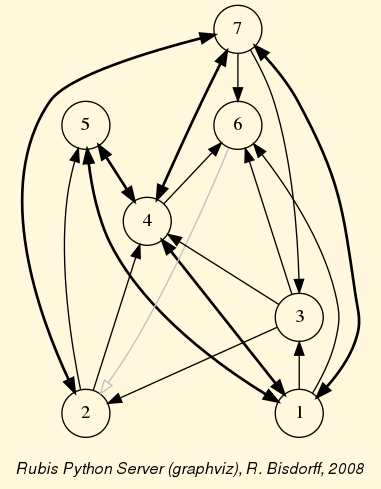
\includegraphics[width=6cm]{Figures/tutRandValDigraph.png}
\caption{The tutorial random valuation digraph. Double links are drawn in bold black with an arrowhead at each end, whereas single asymmetric links are drawn in black with an arrowhead showing the direction of the link. Notice the undetermined relational situation ($r(6\,S\,2) = 0.00$) observed between nodes '6' and '2'. The corresponding link is marked in gray with an open arrowhead in the drawing.}
\label{fig:2.1}       % Give a unique label
\end{figure}
  
\section{Asymmetric and symmetric parts}
\label{sec:2.3}

We may now extract both the \emph{}\emph{symmetric} as well as the asymmetric part of digraph $dg$ with the help of two corresponding constructors (see Listing \ref{list:2.3}).
\begin{lstlisting}[caption={Computing asymmetric and symmetric Parts},label=list:2.3]
>>> from digraphs import AsymmetricPartialDigraph,\
...                      SymmetricPartialDigraph
>>> asymDg = AsymmetricPartialDigraph(rdg)
>>> asymDg.exportGraphViz()
>>> symDg = SymmetricPartialDigraph(rdg)
>>> symDg.exportGraphViz()
\end{lstlisting}
\begin{figure}[h]
%\sidecaption
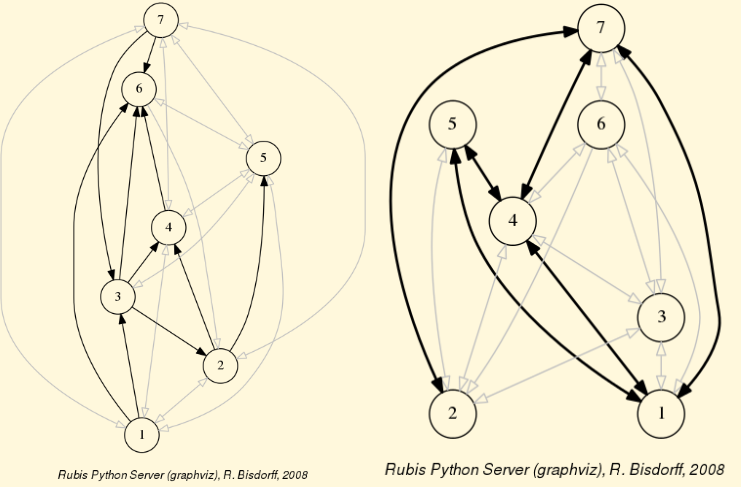
\includegraphics[width=12cm]{Figures/asymSymParts.png}
\caption{Asymmetric and symmetric part of the tutorial random valuation digraph.}
\label{fig:2.2}       % Give a unique label
\end{figure}
The constructor of the partial objects $asymDg$ and $symDg$ puts to the indeterminate characteristic value all not-asymmetric, respectively not-symmetric links between nodes (see Fig. \ref{fig:2.2}).

Here below, for illustration the source code of the {\tt relation} constructor of the {\tt AsymmetricPartialDigraph}\index{AsymmetricPartialDigraph@\texttt{AsymmetricPartialDigraph} class} class.
\begin{lstlisting}[caption={Computing the asymmetric part of a bipolar-valued relation},label=list:2.4,basicstyle=\ttfamily\scriptsize]
def _constructRelation(self):
    actions = self.actions
    Min = self.valuationdomain['min']
    Max = self.valuationdomain['max']
    Med = self.valuationdomain['med']
    relationIn = self.relation
    relationOut = {}
    for a in actions:
	relationOut[a] = {}
	for b in actions:
	    if a != b:
                if relationIn[a][b] >= Med and relationIn[b][a] <= Med:
		    relationOut[a][b] = relationIn[a][b]
		elif relationIn[a][b] <= Med and relationIn[b][a] >= Med:
		    relationOut[a][b] = relationIn[a][b]
		else:
		    relationOut[a][b] = Med
		else:
		    relationOut[a][b] = Med
    return relationOut
\end{lstlisting}

\section{Border and inner parts}
\label{sec:2.4}

We may also extract the border --the part of a digraph induced by the union of its initial and terminal prekernels (see Chapter \ref{sec:17})--  as well as, the inner part -the complement of the border- with the help of two corresponding class constructors: \texttt{GraphBorder}\index{GraphBorder@\texttt{GraphBorder} class} and \texttt{GraphInner}\index{GraphInner@\texttt{GraphInner} class} (see Fig. \ref{fig:2.3}).

Let us illustrate these parts on a linear ordering obtained from the tutorial random valuation digraph $rdg$  with the \NetFlows ranking rule  (see Section \ref{sec:8.3}).  
\begin{lstlisting}[caption={Border and inner part of a linear order},label=list:2.5]
>>> from digraphs import GraphBorder, GraphInner
>>> from linearOrders import NetFlowsOrder
>>> nf = NetFlowsOrder(rdg)
>>> nf.netFlowsOrder
   ['6', '4', '5', '3', '2', '1', '7']
>>> bnf = GraphBorder(nf)
>>> bnf.exportGraphViz(worstChoice=['6'],bestChoice=['7'])
>>> inf = GraphInner(nf)
>>> inf.exportGraphViz(worstChoice=['6'],bestChoice=['7'])
\end{lstlisting}
\begin{figure}[h]
%\sidecaption
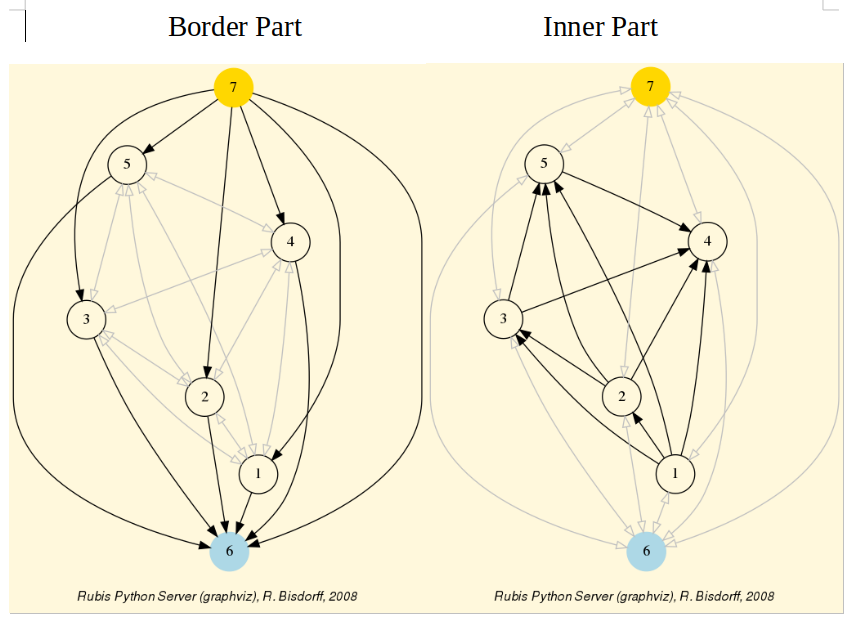
\includegraphics[width=11cm]{Figures/graphBorderAndInner1.png}
\caption{\emph{Border} and \emph{inner} part of a linear order oriented by \emph{terminal} and \emph{initial} kernels.}
\label{fig:2.3}       % Give a unique label
\end{figure}
We may orient the \texttt{graphviz} drawings in Fig. \ref{fig:2.3}  with the terminal node 6 (\texttt{worstChoice} parameter) and initial node 7 (\texttt{bestChoice} parameter) (see Listing \ref{list:2.5} Lines 7 and 9).

The constructor of the partial digraphs $bnf$ and $inf$  (see Lines 3 and 6) puts to the \emph{indeterminate} characteristic value all links not in the \emph{border}, respectively \emph{not} in the \emph{inner} part (see Fig. \ref{fig:2.3}). Being much {\em denser\/} than a linear order, the actual inner part of our tutorial random valuation digraph $dg$ is reduced to a single arc between nodes 3 and 4 (see Fig. \ref{fig:2.4}).
\begin{figure}[h]
%\sidecaption
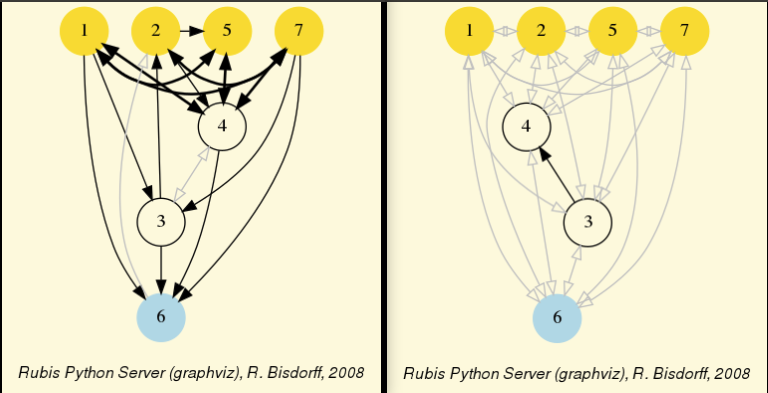
\includegraphics[width=11cm]{Figures/graphBorderAndInner.png}
\caption{Border and inner part of the tutorial random valuation digraph $rdg$.}
\label{fig:2.4}       % Give a unique label
\end{figure}
Indeed, a complete digraph on the limit has no inner part (privacy!) at all, whereas empty and indeterminate digraphs admit both, an empty border and an empty inner part.

\section{Fusion by epistemic disjunction}
\label{sec:2.5}

We may recover object $rdg$ from both partial objects $asymDg$ and $symDg$, or as well from the border $bg$ and the inner part $ig$, with a \emph{bipolar fusion} constructor, also called \emph{epistemic disjunction}, available via the \texttt{FusionDigraph}\index{digraphs!FusionDigraph@\texttt{FusionDigraph}} class. 
\begin{lstlisting}[caption={Epistemic fusion of partial diagraphs},label=list:2.6]
>>> from digraphs import FusionDigraph
>>> fusDg = FusionDigraph(asymDg,symDg,operator='o-max')
>>> # fusDg = FusionDigraph(bg,ig,operator='o-max')
>>> fusDg.showRelationTable()
  * ---- Relation Table -----
   r(xSy) |  '1'    '2'   '3'  '4'   '5'    '6'  '7'	  
   -------|------------------------------------------
    '1'   |  0.00 -0.48  0.70  0.86  0.30  0.38  0.44	 
    '2'   | -0.22  0.00 -0.38  0.50  0.80 -0.54  0.02	 
    '3'   | -0.42  0.08  0.00  0.70 -0.56  0.84 -1.00	 
    '4'   |  0.44 -0.40 -0.62  0.00  0.04  0.66  0.76	 
    '5'   |  0.32 -0.48 -0.46  0.64  0.00 -0.22 -0.52	 
    '6'   | -0.84  0.00 -0.40 -0.96 -0.18  0.00 -0.22	 
    '7'   |  0.88  0.72  0.82  0.52 -0.84  0.04  0.00
\end{lstlisting}
The epistemic fusion operator \texttt{o-max} (see Listing \ref{list:2.6} Line 2) is defined as follows:
\begin{definition}[Disjunctive epistemic fusion]\label{def:disjunctiveFusion}

  Let $r$ and $r'$ characterise two bipolar-valued epistemic situations.
\begin{itemize}
\item $o-max(r, r' ) = \max(r, r' )$ when both $r$ and $r'$ are more or less valid or indeterminate;
\item $o-max(r, r' ) = \min(r, r' )$ when both $r$ and $r'$ are more or less invalid or indeterminate;
\item $o-max(r, r' ) = 0.0$, i.e. indeterminate otherwise.
\end{itemize}
\end{definition}
\section{Dual, converse and codual digraphs}
\label{sec:2.6}

We may as readily compute the \emph{dual} (negated relation \footnote{Not to be confused with the dual graph of a plane graph $g$ that has a vertex for each face of $g$. Here we mean the \emph{less than} (strict converse) relation corresponding to a \emph{greater or equal} relation, or the \emph{less than or equal} relation corresponding to a (strict) \emph{better than} relation.}), the \emph{converse} (transposed relation) and the \emph{codual} (transposed and negated relation) of the digraph instance $rdg$. 
\begin{lstlisting}[caption={Computing associated dual, converse and codual digraphs},label=list:2.7]
>>> from digraphs import DualDigraph, ConverseDigraph, CoDualDigraph
>>> ddg = DualDigraph(rdg)
>>> ddg.showRelationTable()
    -r(xSy) |  '1'    '2'   '3'  '4'   '5'    '6'  '7'	  
    --------|------------------------------------------
    '1 '    |  0.00  0.48 -0.70 -0.86 -0.30 -0.38 -0.44	 
    '2'     |  0.22  0.00  0.38 -0.50  0.80  0.54 -0.02	 
    '3'     |  0.42  0.08  0.00 -0.70  0.56 -0.84  1.00	 
    '4'     | -0.44  0.40  0.62  0.00 -0.04 -0.66 -0.76	 
    '5'     | -0.32  0.48  0.46 -0.64  0.00  0.22  0.52	 
    '6'     |  0.84  0.00  0.40  0.96  0.18  0.00  0.22	 
    '7'     |  0.88 -0.72 -0.82 -0.52  0.84 -0.04  0.00

>>> cdg = ConverseDigraph(rdg)
>>> cdg.showRelationTable()
    * ---- Relation Table -----
     r(ySx) |  '1'    '2'   '3'   '4'   '5'   '6'   '7'	  
    --------|------------------------------------------
    '1'     |  0.00 -0.22 -0.42  0.44  0.32 -0.84  0.88	 
    '2'     | -0.48  0.00  0.08 -0.40 -0.48  0.00  0.72	 
    '3'     |  0.70 -0.38  0.00 -0.62 -0.46 -0.40  0.82	 
    '4'     |  0.86  0.50  0.70  0.00  0.64 -0.96  0.52	 
    '5'     |  0.30  0.80 -0.56  0.04  0.00 -0.18 -0.84	 
    '6'     |  0.38 -0.54  0.84  0.66 -0.22  0.00  0.04	 
    '7'     |  0.44  0.02 -1.00  0.76 -0.52 -0.22  0.00	 

>>> cddg = CoDualDigraph(rdg)
>>> cddg.showRelationTable()
    * ---- Relation Table -----
    -r(ySx) |  '1'    '2'   '3'   '4'   '5'   '6'   '7'	    
    --------|------------------------------------------
    '1'     |  0.00  0.22  0.42 -0.44 -0.32  0.84 -0.88	 
    '2'     |  0.48  0.00 -0.08  0.40  0.48  0.00 -0.72	 
    '3'     | -0.70  0.38  0.00  0.62  0.46  0.40 -0.82	 
    '4'     | -0.86 -0.50 -0.70  0.00 -0.64  0.96 -0.52	 
    '5'     | -0.30 -0.80  0.56 -0.04  0.00  0.18  0.84	 
    '6'     | -0.38  0.54 -0.84 -0.66  0.22  0.00 -0.04	 
    '7'     | -0.44 -0.02  1.00 -0.76  0.52  0.22  0.00	 
\end{lstlisting}
  
Computing the dual, respectively the converse of a dograph, may also be done with prefixing the \texttt{\_\_neg\_\_} ($-$) or the \texttt{\_\_invert\_\_} ($\sim$) operator. The codual of a \texttt{Digraph} object may, hence, as well be computed with a \emph{composition} (in either order) of both operations.
\begin{lstlisting}[caption={Computing the dual, the converse and the codual of a digraph},label=list:2.8]
>>> ddg = -rdg   # dual of rdg
>>> cdg = ~rdg   # converse of rdg
>>> cddg = ~(-rdg) # = -(~(rdg) codual of rdg
>>> (-(~rdg)).showRelationTable()
  * ---- Relation Table -----
   -r(ySx) |  '1'    '2'   '3'   '4'   '5'   '6'   '7'	    
   --------|------------------------------------------
   '1'     |  0.00  0.22  0.42 -0.44 -0.32  0.84 -0.88	 
   '2'     |  0.48  0.00 -0.08  0.40  0.48  0.00 -0.72	 
   '3'     | -0.70  0.38  0.00  0.62  0.46  0.40 -0.82	 
   '4'     | -0.86 -0.50 -0.70  0.00 -0.64  0.96 -0.52	 
   '5'     | -0.30 -0.80  0.56 -0.04  0.00  0.18  0.84	 
   '6'     | -0.38  0.54 -0.84 -0.66  0.22  0.00 -0.04	 
   '7'     | -0.44 -0.02  1.00 -0.76  0.52  0.22  0.00	 
\end{lstlisting}
  
\section{Symmetric and transitive closures}
\label{sec:2.7}

Symmetric and transitive closures, by default in-site constructors, are also available (see Fig. \ref{fig:2.5}). Note that it is a good idea, before going ahead with these in-site operations, who irreversibly modify the original $rdg$ object, to previously make a backup version of $rdg$. The simplest storage method, always provided by the generic \texttt{Digraph.save()}, writes out in a named file the python content of the Digraph object in string representation (see Section \ref{sec:1.3}).
\begin{lstlisting}[caption={Symmeric and transitive closures},label=list:2.9]
>>> rdg.save('tutRandValDigraph')
>>> rdg.closeSymmetric(InSite=True)
>>> rdg.closeTransitive(InSite=True)
>>> rdg.exportGraphViz('strongComponents')
\end{lstlisting}
\begin{figure}[h]
\sidecaption[t]
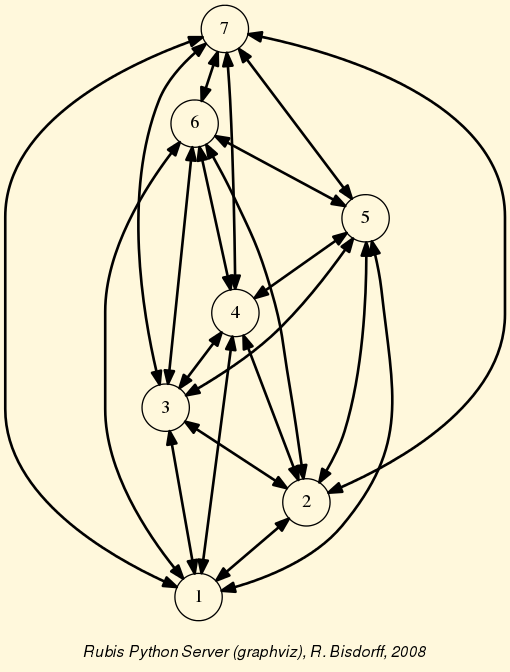
\includegraphics[width=6cm]{Figures/strongComponents.png}
\caption{Symmetric and transitive closure of the tutorial random valuation digraph $rdg$.}
\label{fig:2.5}       % Give a unique label
\end{figure}

The \texttt{closeSymmetric()}\index{digraphs!Digraph!closeSymmetric@\texttt{closeSymmetric()}} method (see Listing \ref{list:2.9}  Line 2), of complexity $O(n^2)$ where $n$ denotes the digraph's order, changes, on the one hand, all single pairwise links it may detect into double links by operating a disjunction of the pairwise relations. On the other hand, the \texttt{closeTransitive()}\index{digraphs!Digraph!closeTransitive@\texttt{closeTransitive()}}  method (see Line 3), implements the \emph{Roy-Warshall} transitive closure algorithm of complexity $O(n^3)$ \footnote{\citet{ROY-1959}\index{Roy@\textsl{B. Roy}} and \citet{WAR-1962}\index{warshall@\textsl{S. Warshall}}.}.

The same \texttt{closeTransitive()} with a \texttt{Reverse = True} flag may be readily used for eliminating all transitive arcs from a transitive digraph instance. We make usage of this feature when drawing Hasse diagrams of \texttt{TransitiveDigraph}\index{transitiveDigraphs@\texttt{transitiveDigraphs}!TransitiveDigraph@\texttt{TransitiveDigraph}} objects.

\section{Strong components}
\label{sec:2.8}

As the original digraph $rdg$ was connected (see above the result of the showShort() command), both the symmetric and the transitive closures operated together, will necessarily produce a single strong component, i.e. a \textbf{complete} digraph. We may sometimes wish to collapse all strong components in a given digraph and construct the so \emph{collapsed} digraph. Using the \texttt{StrongComponentsCollapsedDigraph} constructor \index{digraphs!StrongComponentsCollapsedDigraph@\texttt{StrongComponentsCollapsedDigraph}} here will render a single hyper-node gathering all the original nodes (see Line 7 below).
\begin{lstlisting}[caption={Computing the strong components in a digraph},label=list:2.10]
>>> from digraphs import StrongComponentsCollapsedDigraph
>>> sc = StrongComponentsCollapsedDigraph(dg)
>>> sc.showAll()
  *----- show detail -----*
   Digraph          : tutRandValDigraph_Scc
  *---- Actions ----*
    ['_7_1_2_6_5_3_4_']
  *---- Relation Table -----
      S     |  'Scc_1'	  
     -------|---------
     'Scc_1' |  0.00
  *---- strong Components ----*
   short 	 content
   'Scc_1' 	 '_7_1_2_6_5_3_4_'
  *---- Neighborhoods ----*
   Gamma     :
   'frozenset({'7','1','2','6','5','3','4'})':
                     in => set(), out => set()
   Not Gamma :
   'frozenset({'7','1','2','6','5','3','4'})':
                     in => set(), out => set()
\end{lstlisting}
  
\section{CSV storage}
\label{sec:2.9}

Sometimes it is required to exchange the graph valuation data in CSV format with a statistical package like \textbf{R}\footnote{\url{https://www.r-project.org/}}. For this purpose it is possible to export the digraph data into a CSV file. The valuation domain is hereby normalized by default to the range $[-1.0,1.0]$ and the diagonal is put by default to the minimal value $-1.0$.
\begin{lstlisting}
>>> rdg = Digraph('tutRandValDigraph')
>>> rdg.saveCSV('tutRandValDigraph')
  # content of file tutRandValDigraph.csv
  "d","1","2","3","4","5","6","7"
  "1",-1.0,0.48,-0.7,-0.86,-0.3,-0.38,-0.44
  "2",0.22,-1.0,0.38,-0.5,-0.8,0.54,-0.02
  "3",0.42,-0.08,-1.0,-0.7,0.56,-0.84,1.0
  "4",-0.44,0.4,0.62,-1.0,-0.04,-0.66,-0.76
  "5",-0.32,0.48,0.46,-0.64,-1.0,0.22,0.52
  "6",0.84,0.0,0.4,0.96,0.18,-1.0,0.22
  "7",-0.88,-0.72,-0.82,-0.52,0.84,-0.04,-1.0
\end{lstlisting}
  
It is possible to reload a \texttt{Digraph} instance from its previously saved CSV file content.
\begin{lstlisting} 
>>> from digraphs import CSVDigraph   
>>> rdgcsv = CSVDigraph('tutRandValDigraph')
>>> rdgcsv.showRelationTable(ReflexiveTerms=False)
    * ---- Relation Table -----
    r(xSy) |   '1'   '2'   '3'   '4'   '5'   '6'   '7'	  
    -------|------------------------------------------------------------
    '1'    |   -   -0.48  0.70  0.86  0.30  0.38  0.44	 
    '2'    | -0.22   -   -0.38  0.50  0.80 -0.54  0.02	 
    '3'    | -0.42  0.08   -    0.70 -0.56  0.84 -1.00	 
    '4'    |  0.44 -0.40 -0.62   -    0.04  0.66  0.76	 
    '5'    |  0.32 -0.48 -0.46  0.64   -   -0.22 -0.52	 
    '6'    | -0.84  0.00 -0.40 -0.96 -0.18   -   -0.22	 
    '7'    |  0.88  0.72  0.82  0.52 -0.84  0.04   -
\end{lstlisting}
  
It is as well possible to show a colored version of the valued relation table in a system browser window tab (see Fig. \ref{fig:2.5}).
\begin{lstlisting}
>>> rdgcsv.showHTMLRelationTable(tableTitle="Tutorial random digraph")
\end{lstlisting}
 \begin{figure}[h]
\sidecaption
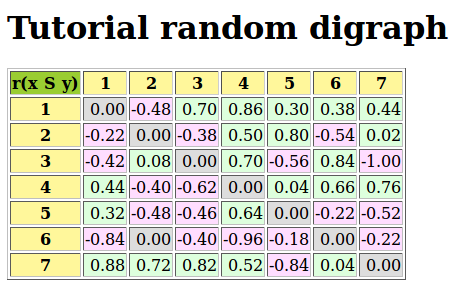
\includegraphics[width=7cm]{Figures/htmlTutorialDigraph.png}
\caption{The valued relation table shown in a browser window. Positive arcs are shown in green and negative arcs in red. Indeterminate --zero-valued-- links, like the reflexive diagonal ones or the link between node '6' and node '2', are shown in gray.}
\label{fig:2.6}       % Give a unique label
\end{figure}
 
\section{Complete, empty and indeterminate digraphs}
\label{sec:2.10}

Let us finally mention some special universal classes of digraphs that are readily available in the \texttt{digraphs} module\footnote{See \citealp{BIS-2021}}, like the \texttt{CompleteDigraph}\index{digraphs!CompleteDigraph@\texttt{Complete \index{digraphs@\texttt{digraphs}|StrongComponentsCollapsedDigraph@\texttt{StrongComponentsCollapsedDigraph}} Digraph}}, the \texttt{EmptyDigraph}\index{digraphs!EmptyDigraph@\texttt{EmptyDigraph}} and the \texttt{IndeterminateDigraph}\index{digraphs!IndeterminateDigraph@\texttt{IndeterminateDigraph}} classes, which put all characteristic values respectively to the maximum, the minimum or the median indeterminate characteristic value.
\begin{lstlisting}[caption={Complete, empty and indeterminate digraphs},label=list:2.11]
>>> from digraphs import CompleteDigraph,EmptyDigraph,\
...   			 IndeterminateDigraph
   
>>> e = EmptyDigraph(order=5)
>>> e.showRelationTable()
    * ---- Relation Table -----
      S   |    '1'    '2'    '3'    '4'	   '5'	  
    ---- -|-----------------------------------
    '1'   |  -1.00  -1.00  -1.00  -1.00	 -1.00	 
    '2'   |  -1.00  -1.00  -1.00  -1.00	 -1.00	 
    '3'   |  -1.00  -1.00  -1.00  -1.00	 -1.00	 
    '4'   |  -1.00  -1.00  -1.00  -1.00	 -1.00	 
    '5'   |  -1.00  -1.00  -1.00  -1.00	 -1.00

>>> e.showNeighborhoods() 
    Neighborhoods:
      Gamma     :
    '1': in => set(), out => set()
    '2': in => set(), out => set()
    '5': in => set(), out => set()
    '3': in => set(), out => set()
    '4': in => set(), out => set()
      Not Gamma :
    '1': in => {'2', '4', '5', '3'}, out => {'2', '4', '5', '3'}
    '2': in => {'1', '4', '5', '3'}, out => {'1', '4', '5', '3'}
    '5': in => {'1', '2', '4', '3'}, out => {'1', '2', '4', '3'}
    '3': in => {'1', '2', '4', '5'}, out => {'1', '2', '4', '5'}
    '4': in => {'1', '2', '5', '3'}, out => {'1', '2', '5', '3'}

>>> i = IndeterminateDigraph()
    * ---- Relation Table -----
      S   |   '1'   '2'	  '3'	'4'   '5'	  
    ------|------------------------------
    '1'   |  0.00  0.00	 0.00  0.00  0.00	 
    '2'   |  0.00  0.00	 0.00  0.00  0.00	 
    '3'   |  0.00  0.00	 0.00  0.00  0.00	 
    '4'   |  0.00  0.00	 0.00  0.00  0.00	 
    '5'   |  0.00  0.00	 0.00  0.00  0.00	 

>>> i.showNeighborhoods()
    Neighborhoods:
      Gamma     :
    '1': in => set(), out => set()
    '2': in => set(), out => set()
    '5': in => set(), out => set()
    '3': in => set(), out => set()
    '4': in => set(), out => set()
      Not Gamma :
    '1': in => set(), out => set()
    '2': in => set(), out => set()
    '5': in => set(), out => set()
    '3': in => set(), out => set()
    '4': in => set(), out => set()
\end{lstlisting}

Mind the subtle difference between the neighborhoods of an \textbf{empty} and the neighborhoods of an \textbf{indeterminate} digraph instance. In the first kind, the neighborhoods are known to be completely \emph{empty}  (see Listing \ref{list:2.11} Lines 22-27) whereas, in the latter, \emph{nothing is known} about the actual neighborhoods of the nodes  (see Lines 45-50). These two cases illustrate why in the case of \textbf{bipolar-valued} digraphs, we may need both a \texttt{gamma} \textbf{and} a \texttt{notGamma} attribute.

%%%%%%% The chapter bibliography
%\normallatexbib
\clearpage
%\phantomsection
%\addcontentsline{toc}{section}{Chapter Bibliograhy}
\bibliographystyle{spbasic}
%\typeout{}
\bibliography{03-backMatters/reference}
%\chapter{Working with bipolar-valued digraphs}
\label{sec:2}

\abstract*{ The chapter introduces bipolar-valued digraphs, the fondamental root type of all the specialised digraphs implemented in the \Digraph modules. With the help of a randomly valued digraph, we illustrate some basic digraph manipulation methods, like drawing the digraph, dividing the digraph into its asymmetric and symmetric parts, separating the border from the inner part, computing associated dual, converse and codual digraphs, and operating symmetric and transitive closures.}

\abstract{ The chapter introduces bipolar-valued digraphs, the fondamental root type of all the specialised digraphs implemented in the \Digraph modules. With the help of a randomly valued digraph, we illustrate some basic digraph manipulation methods, like drawing the digraph, dividing the digraph into its asymmetric and symmetric parts, separating the border from the inner part, computing associated dual, converse and codual digraphs, and operating symmetric and transitive closures.}

\section{Random bipolar-valued digraphs}

In Listing~\vref{list:2.1}, we generate a uniformly random $[-1.0; +1.0]$-valued digraph of order 7, denoted \texttt{rdg} and modelling, for instance, a binary relation $S(x,y)$ defined on the set of nodes of \texttt{rdg}. For this purpose, the \Digraph resources provide in the \texttt{randomDigraphs}\index{randomDigraphs@\texttt{randomDigraphs} module} module a specific \texttt{RandomValuationDigraph}\index{RandomValuationDigraph@\texttt{RandomValuationDigraph} class} class \citep{BIS-2021b}.
\begin{lstlisting}[caption={Random bipolar-valued digraph instance},label=list:2.1]
>>> from randomDigraphs import RandomValuationDigraph
>>> rdg = RandomValuationDigraph(order=7)
>>> rdg.save('tutRandValDigraph')
>>> from digraphs import Digraph
>>> rdg = Digraph('tutRandValDigraph')
>>> rdg
  *------- Digraph instance description ------*
   Instance class      : Digraph
   Instance name       : tutRandValDigraph
   Digraph Order       : 7
   Digraph Size        : 22
   Valuation domain    : [-1.00;1.00]
   Determinateness (%) : 75.24
   Attributes          : ['name','actions','order',
                          'valuationdomain','relation',
                          'gamma','notGamma']
\end{lstlisting}   

With the \texttt{save()} \index{save@\texttt{save()}} method (see Line 3) we keep for future use a backup version of \texttt{rdg} which is saved into a file named \texttt{tutRandValDigraph.py} in the current working directory. The genuine \texttt{Digraph} class constructor may restore the \texttt{rdg} object from the stored file (Lines 4-5). We may easily inspect the content of \texttt{rdg} (Line 6). The digraph size 22 indicates the number of positively valued arcs. The valuation domain is uniformly distributed in the interval $[-1.0; 1.0]$ and the mean absolute arc valuation is $(0.7524 \times 2)\, -\, 1.0 \;=\; 0.5048$ (Line 13).

As mentioned in the previous Chapter~\ref{sec:1}, all objects of \texttt{Digraph} type contain at least the list of attributes shown here in Lines 14-16: --a \texttt{name} (string), --a dictionary of \texttt{actions} (digraph nodes), --an \texttt{order} (integer) attribute containing the number of actions, --a \texttt{valuationdomain} dictionary, --a double dictionary \texttt{relation} representing the adjacency table of the digraph relation, --a \texttt{gamma} and --a {\tt notGamma} dictionary containing the direct neighbourhood of each action.

The \texttt{Digraph} class provides some generic \texttt{show...()} methods for exploring the content of a given \texttt{ Digraph} object, like the \texttt{showRelationTable()}\index{showRelationTable@\texttt{showRelationTable()}}, the \texttt{showComponents()}\index{showComponents@\texttt{showComponents()}} and the \texttt{showNeighborhoods()}\index{showNeighborhoods@\texttt{showNeighborhoods()}} methods.
\begin{lstlisting}[caption={Example of random valuation digraph},label=list:2.2]
>>> rdg.showRelationTable()
  * ---- Relation Table -----
   r(xSy) |  '1'    '2'   '3'  '4'   '5'    '6'  '7'	  
   -------|-------------------------------------------
    '1'   |  0.00 -0.48  0.70  0.86  0.30  0.38  0.44	 
    '2'   | -0.22  0.00 -0.38  0.50  0.80 -0.54  0.02	 
    '3'   | -0.42  0.08  0.00  0.70 -0.56  0.84 -1.00	 
    '4'   |  0.44 -0.40 -0.62  0.00  0.04  0.66  0.76	 
    '5'   |  0.32 -0.48 -0.46  0.64  0.00 -0.22 -0.52	 
    '6'   | -0.84  0.00 -0.40 -0.96 -0.18  0.00 -0.22	 
    '7'   |  0.88  0.72  0.82  0.52 -0.84  0.04  0.00
>>> rdg.showComponents()
  *--- Connected Components ---*
  1: ['1', '2', '3', '4', '5', '6', '7']
>>> rdg.showNeighborhoods()
  *---- Neighborhoods ------*
     Gamma:
     '1': in => {'5','7','4'}, out => {'5','7','6','3','4'}
     '2': in => {'7','3'},out => {'5','7','4'}
     '3': in => {'7','1'}, out => {'6','2','4'}
     '4': in => {'5','7','1','2','3'}, out => {'5','7','1','6'}
     '5': in => {'1','2','4'}, out => {'1','4'}
     '6': in => {'7','1','3','4'}, out => set()
     '7': in => {'1','2','4'}, out => {'1','2','3','4','6'}
     Not Gamma:
     '1': in => {'6','2','3'}, out => {'2'}
     '2': in => {'5','1','4'}, out => {'1','6','3'}
     '3': in => {'5','6','2','4'}, out => {'5','7','1'}
     '4': in => {'6'}, out => {'2','3'}
     '5': in => {'7','6','3'}, out => {'7','6','2','3'}
     '6': in => {'5','2'}, out => {'5','7','1','3','4'}
     '7': in => {'5','6','3'}, out => {'5'}
\end{lstlisting}   

Mind that some \texttt{Digraph} class methods will ignore the \emph{reflexive} links by considering that they are \emph{indeterminate}, i.e. the characteristic value $r(x\,S\,x)$ for all action $x$ is set to the \emph{median}, i.e. \emph{indeterminate} value $0.0$ in this case (see Listing~\vref{list:2.2} Lines 5-11 and \citet{BIS-2004a}).

\section{Graphviz drawings}
\label{sec:2.2}

An even better insight into the \texttt{Digraph} object \texttt{rdg} is given by looking at its \href{https://graphviz.org/}{graphviz} drawing \citep{graphviz}\footnote{The \texttt{exportGraphViz()} method is depending on drawing tools from the graphviz software (https://graphviz.org/). On Linux Ubuntu or Debian you may try \texttt{sudo apt-get install graphviz} to install them. There are ready \emph{dmg} installers for Mac OSX.}\index{graphviz}.
\begin{lstlisting}
>>> rdg.exportGraphViz('tutRandValDigraph')
 *---- exporting a dot file for GraphViz tools ------*
  Exporting to tutRandValDigraph.dot
  dot -Grankdir=BT -Tpng tutRandValDigraph.dot\
                           -o tutRandValDigraph.png
\end{lstlisting}
\begin{figure}[ht]
\sidecaption[t]
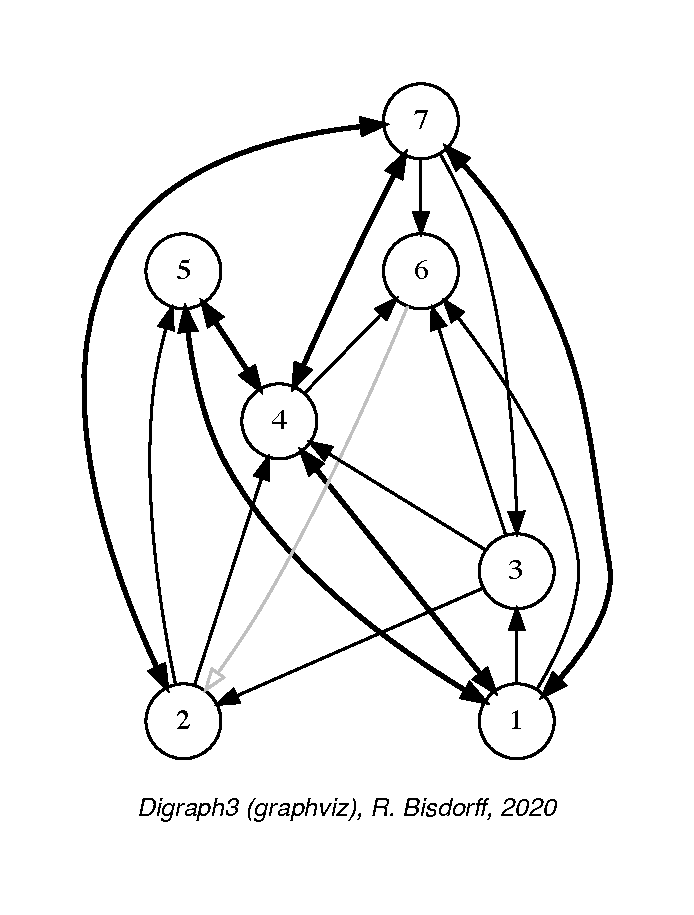
\includegraphics[width=6cm]{Figures/2-1-tutRandValDigraph.pdf}
\caption{\emph{The tutorial random valuation digraph}. Double links are drawn in bold black with an arrowhead at each end, whereas single asymmetric links are drawn in black with an arrowhead showing the direction of the link. Notice the undetermined relational situation ($r(6\,S\,2) = 0.00$) observed between nodes '6' and '2'. The corresponding link is marked in gray with an open arrowhead in the drawing}
\label{fig:2.1}       % Give a unique label
\end{figure}
  
\section{Asymmetric and symmetric parts}
\label{sec:2.3}

We may now extract both the \emph{}\emph{symmetric} as well as the \emph{asymmetric} part of digraph \texttt{rdg} with the help of two corresponding constructors (see List.~\vref{list:2.3}) \index{AsymmetricPartialDigraph@\texttt{AsymmetricPartialDigraph} class}\index{SymmetricPartialDigraph@\texttt{SymmetricPartialDigraph} class}.
\begin{lstlisting}[caption={Computing asymmetric and symmetric Parts},label=list:2.3]
>>> from digraphs import AsymmetricPartialDigraph,\
...                      SymmetricPartialDigraph
>>> asymDg = AsymmetricPartialDigraph(rdg)
>>> asymDg.exportGraphViz()
>>> symDg = SymmetricPartialDigraph(rdg)
>>> symDg.exportGraphViz()
\end{lstlisting}
\begin{figure}[ht]
  % \sidecaption
  Asymmetric Part \hfill Symmetric Part \\
  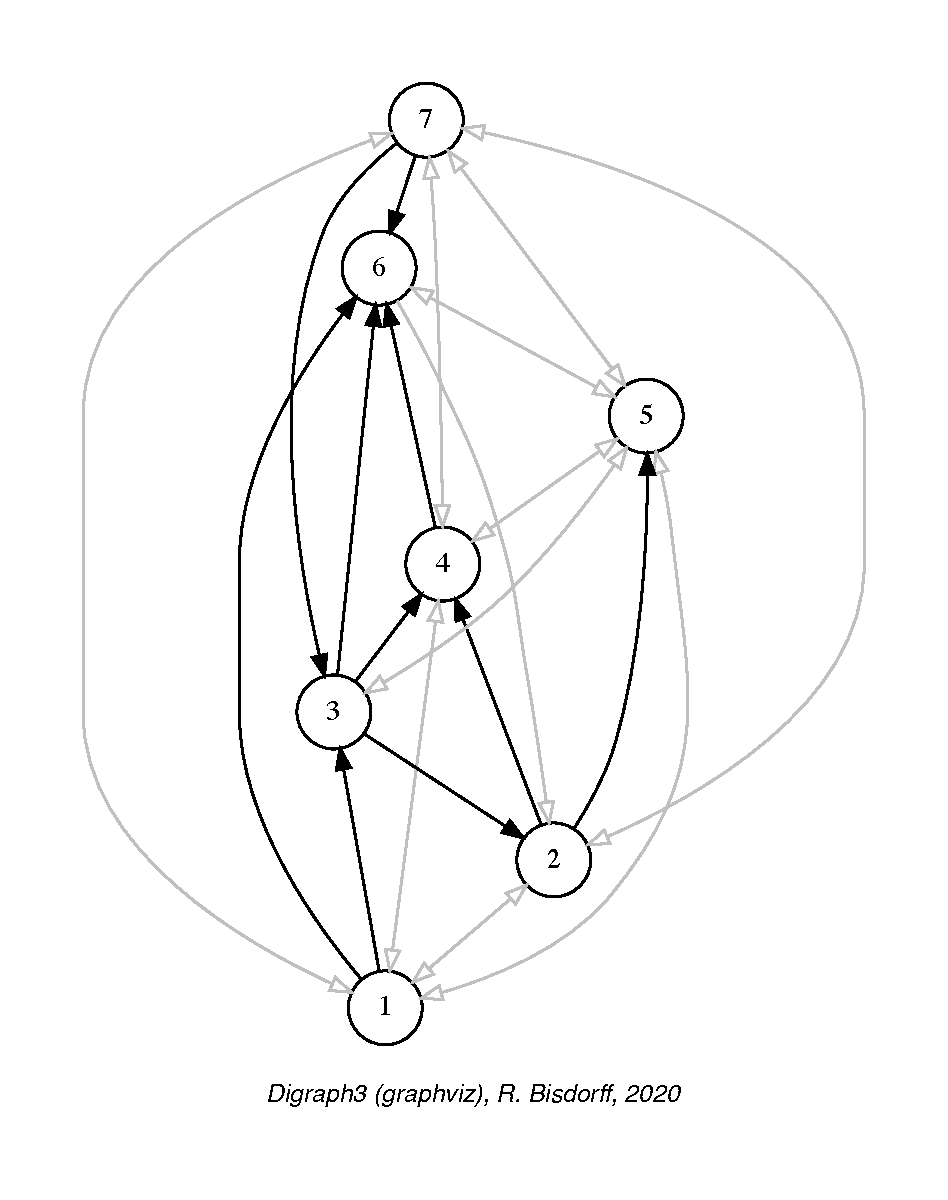
\includegraphics[height=6cm]{Figures/2-2-asymmetricPart.pdf}\hfill
  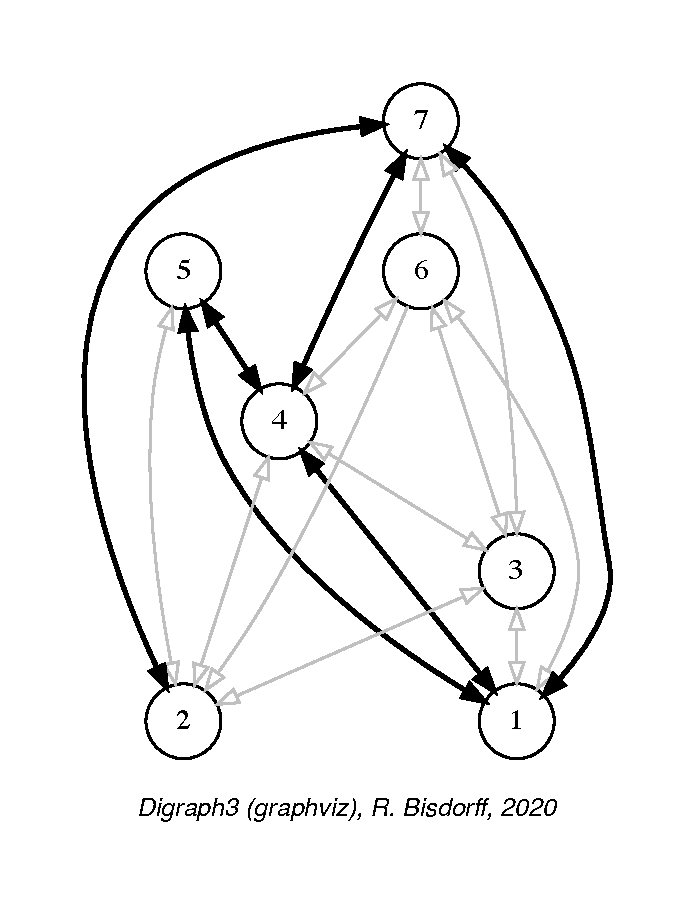
\includegraphics[height=6cm]{Figures/2-2-symmetricPart.pdf}\hfill
\caption{Asymmetric and symmetric part of the tutorial random valuation digraph}
\label{fig:2.2}       % Give a unique label
\end{figure}

The constructor of the partial objects \texttt{asymDg} and \texttt{symDg} puts to the indeterminate characteristic value all non-asymmetric, respectively non-symmetric links between nodes (see Fig.~\vref{fig:2.2}).

Here below, for illustration the source code of the \texttt{ relation} constructor of the \texttt{AsymmetricPartialDigraph} class.
\begin{lstlisting}[caption={Computing the asymmetric part of a bipolar-valued relation},label=list:2.4,basicstyle=\ttfamily\scriptsize]
def _constructRelation(self):
    actions = self.actions
    Min = self.valuationdomain['min']
    Max = self.valuationdomain['max']
    Med = self.valuationdomain['med']
    relationIn = self.relation
    relationOut = {}
    for a in actions:
	relationOut[a] = {}
	for b in actions:
	    if a != b:
                if relationIn[a][b] >= Med and relationIn[b][a] <= Med:
		    relationOut[a][b] = relationIn[a][b]
		elif relationIn[a][b] <= Med and relationIn[b][a] >= Med:
		    relationOut[a][b] = relationIn[a][b]
		else:
		    relationOut[a][b] = Med
	    else: # reflexive links are ignored
		relationOut[a][b] = Med
    return relationOut
\end{lstlisting}

\section{Border and inner parts}
\label{sec:2.4}

We may also extract the \emph{border} --the part of a digraph induced by the union of its initial and terminal prekernels (see Chap.~\ref{sec:17})--  as well as, the \emph{inner part} --the complement of the border-- with the help of two corresponding class constructors: \texttt{GraphBorder}\index{GraphBorder@\texttt{GraphBorder} class} and \texttt{GraphInner}\index{GraphInner@\texttt{GraphInner} class} (see Fig.~\vref{fig:2.3}).

\begin{figure}[ht]
%\sidecaption
  Border Part \hfill Inner Part \\
  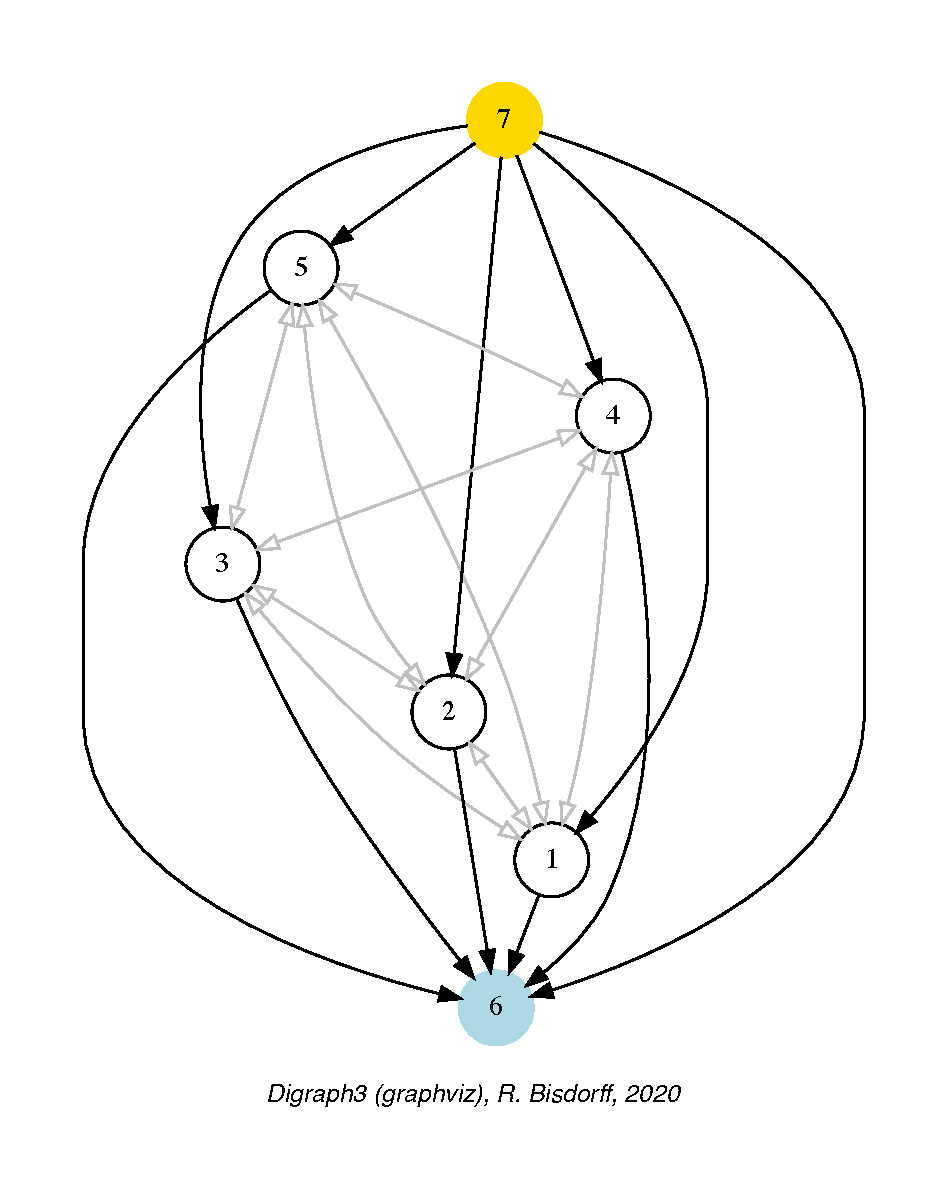
\includegraphics[height=6cm]{Figures/2-3-linearOrderBorder.pdf}\hfill
  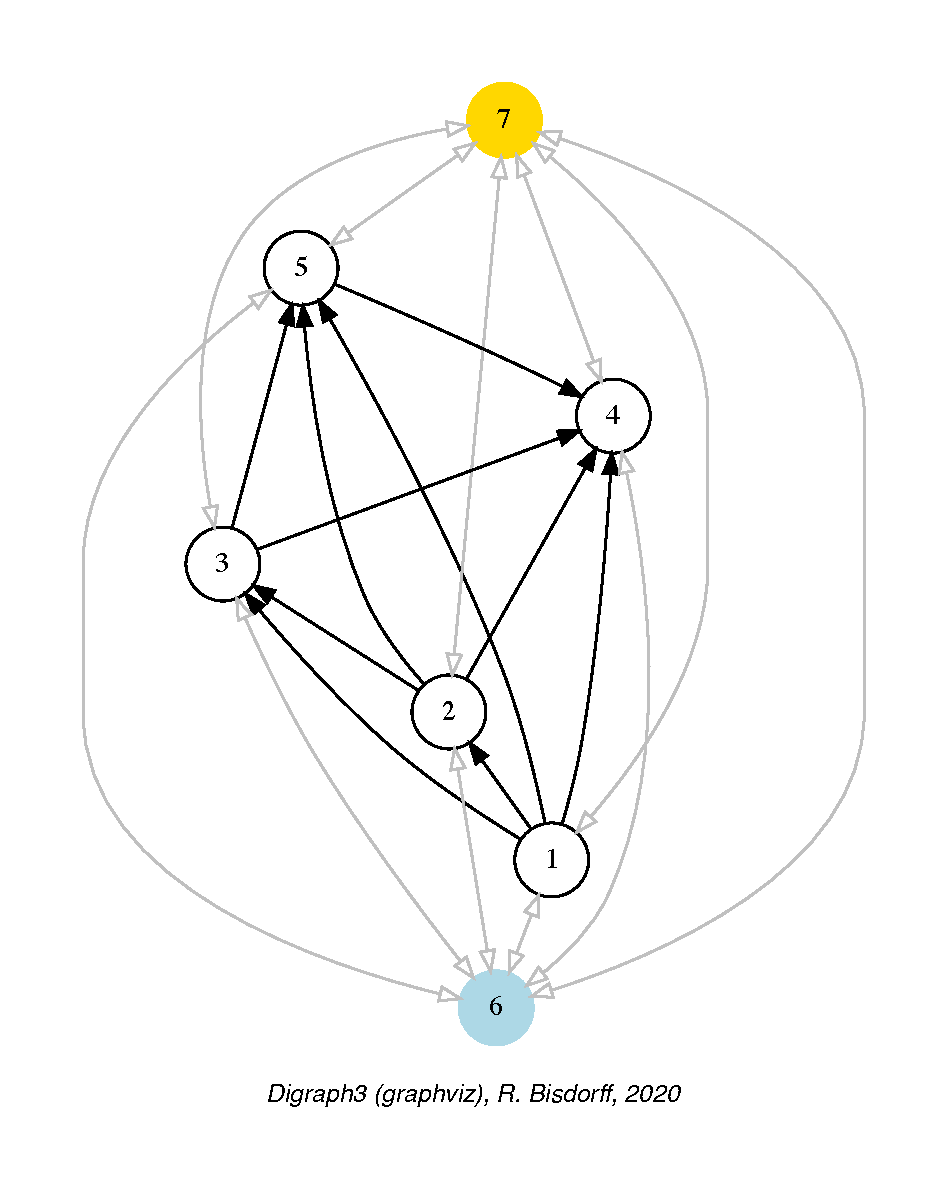
\includegraphics[height=6cm]{Figures/2-3-linearOrderInner.pdf}\hfill
\caption{\emph{Border} and \emph{inner} part of a linear order oriented by \emph{terminal} and \emph{initial} kernels.}
\label{fig:2.3}       % Give a unique label
\end{figure}
Let us illustrate the digraph border and inner parts on a linear ordering obtained from the tutorial random valuation digraph \texttt{rdg}  with the \NetFlows ranking rule  (see Sec.~\ref{sec:8.3}).  
\begin{lstlisting}[caption={Border and inner part of a linear order},label=list:2.5]
>>> from digraphs import GraphBorder, GraphInner
>>> from linearOrders import NetFlowsOrder
>>> nf = NetFlowsOrder(rdg)
>>> nf.netFlowsOrder
   ['6', '4', '5', '3', '2', '1', '7']
>>> bnf = GraphBorder(nf)
>>> bnf.exportGraphViz(lastChoice=['6'],firstChoice=['7'])
>>> inf = GraphInner(nf)
>>> inf.exportGraphViz(lastChoice=['6'],firstChoice=['7'])
\end{lstlisting}
We may orient the \texttt{graphviz} drawings in Figure~\vref{fig:2.3}  with the terminal node 6 (\texttt{lastChoice} parameter) and initial node 7 (\texttt{firstChoice} parameter) (see List.~\vref{list:2.5} Lines 7 and 9).

The constructor of the partial digraphs \texttt{bnf} and \texttt{inf}  (see Lines 3 and 6) puts to the \emph{indeterminate} characteristic value all links not in the \emph{border}, respectively \emph{not} in the \emph{inner} part (see Fig.~\vref{fig:2.3}). Being much {\em denser\/} than a linear order, the actual inner part of our tutorial random valuation digraph \texttt{rdg} is reduced to a single arc between nodes 3 and 4 (see Fig.~\vref{fig:2.4}). Indeed, a complete digraph on the limit has no inner part (privacy!) at all, whereas empty and indeterminate digraphs admit both, an empty border and an empty inner part.
\begin{figure}[h]
%\sidecaption
  Border Part \hfill Inner Part \\
  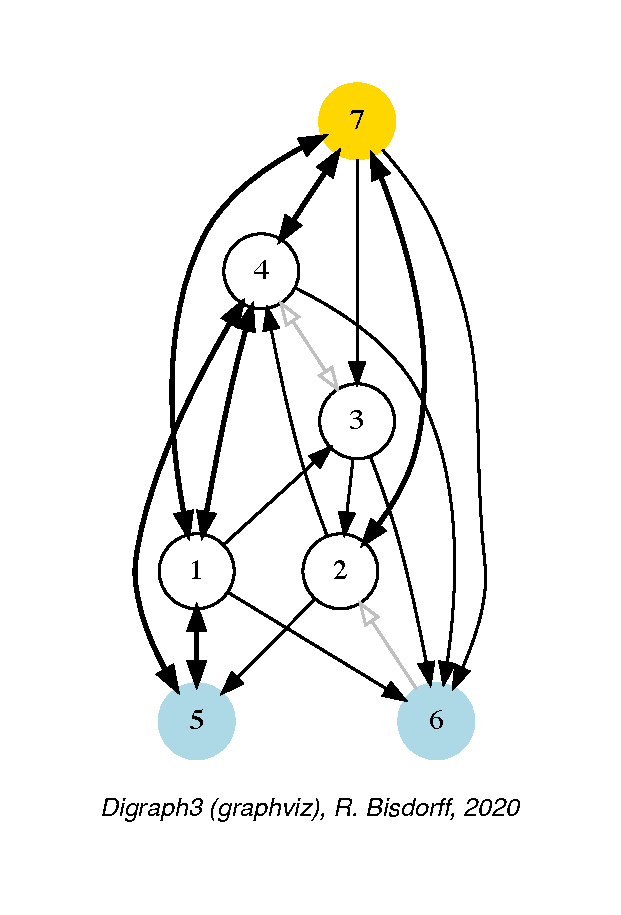
\includegraphics[height=6cm]{Figures/2-4-tutRandValDigraph_border.pdf}\hfill
  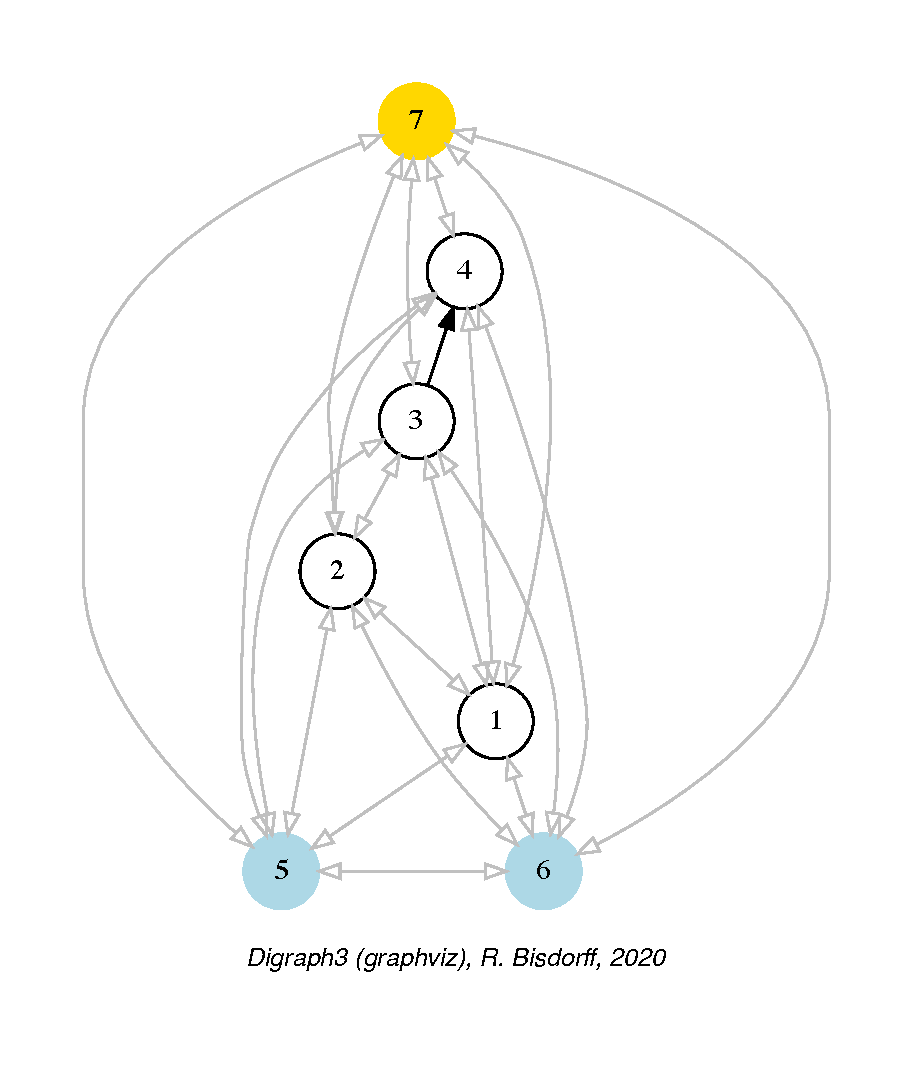
\includegraphics[height=6cm]{Figures/2-4-tutRandValDigraph_inner.pdf}\hfill
\caption{Border and inner part of the tutorial random valuation digraph \texttt{rdg}}
\label{fig:2.4}       % Give a unique label
\end{figure}

\section{Fusion by epistemic disjunction}
\label{sec:2.5}

We may recover object \texttt{rdg} from both partial objects \texttt{asymDg} and \texttt{symDg}, or as well from the border \texttt{bg} and the inner part \texttt{ig}, with a \emph{bipolar fusion} operator, also called \emph{epistemic disjunction}, available via the \texttt{FusionDigraph}\index{FusionDigraph@\texttt{FusionDigraph} class} class. 
\begin{lstlisting}[caption={Epistemic fusion of partial diagraphs},label=list:2.6]
>>> from digraphs import FusionDigraph
>>> fusDg = FusionDigraph(asymDg,symDg,operator='o-max')
>>> # fusDg = FusionDigraph(bg,ig,operator='o-max')
>>> fusDg.showRelationTable()
  * ---- Relation Table -----
   r(xSy) |  '1'    '2'   '3'  '4'   '5'    '6'  '7'	  
   -------|------------------------------------------
    '1'   |  0.00 -0.48  0.70  0.86  0.30  0.38  0.44	 
    '2'   | -0.22  0.00 -0.38  0.50  0.80 -0.54  0.02	 
    '3'   | -0.42  0.08  0.00  0.70 -0.56  0.84 -1.00	 
    '4'   |  0.44 -0.40 -0.62  0.00  0.04  0.66  0.76	 
    '5'   |  0.32 -0.48 -0.46  0.64  0.00 -0.22 -0.52	 
    '6'   | -0.84  0.00 -0.40 -0.96 -0.18  0.00 -0.22	 
    '7'   |  0.88  0.72  0.82  0.52 -0.84  0.04  0.00
\end{lstlisting}

The epistemic fusion operator \texttt{o-max} (see List.~\vref{list:2.6} Line 2) is defined as follows:
\begin{definition}[Disjunctive epistemic fusion operator \texttt{o-max}]\label{def:disjunctiveFusion}

\noindent Let $r$ and $r'$ characterise two bipolar-valued epistemic situations:
\begin{itemize}[leftmargin=0.5cm,rightmargin=0.5cm,nosep]
\item \texttt{o-max}$(r, r')$ = $\max(r, r' )$ when both $r$ and $r'$ are more or less valid or indeterminate;
\item \texttt{o-max}$(r, r')$ = $\min(r, r' )$ when both $r$ and $r'$ are more or less invalid or indeterminate;
\item \texttt{o-max}$(r, r')$ = $0.0$, i.e. indeterminate otherwise.
\end{itemize}
\end{definition}

Mind that the \texttt{o-max} operator, like a mean operator, is \emph{not associative} when more than 2 operands are given. In order to make the \texttt{o-max} fusion univocal, the following rule is applied: --first, all positive and negative terms are separately aggregated, --then the \texttt{o-max} fusion is applied on both aggregates.

\section{Dual, converse and codual digraphs}
\label{sec:2.6}

We may as readily compute the \emph{dual}\index{DualDigraph@\texttt{DualDigraph} class} (negated relation \footnote{Not to be confused with the dual graph of a plane graph $g$ that has a vertex for each face of $g$. Here we mean the \emph{less than} (strict converse) relation corresponding to a \emph{greater or equal} relation, or the \emph{less than or equal} relation corresponding to a (strict) \emph{better than} relation.}), the \emph{converse}\index{ConverseDigraph@\texttt{ConverseDigraph} class} (transposed relation) and the \emph{codual}\index{CoDualDigraph@\texttt{CoDualDigraph} class} (transposed and negated relation) of the digraph instance \texttt{rdg}. 
\begin{lstlisting}[caption={Computing associated dual, converse and codual digraphs},label=list:2.7]
>>> from digraphs import\
...          DualDigraph, ConverseDigraph, CoDualDigraph
>>> # dual of rdg
>>> ddg = DualDigraph(rdg)
>>> ddg.showRelationTable()
    -r(xSy) |  '1'    '2'   '3'  '4'   '5'    '6'  '7'	  
    --------|------------------------------------------
    '1 '    |  0.00  0.48 -0.70 -0.86 -0.30 -0.38 -0.44	 
    '2'     |  0.22  0.00  0.38 -0.50  0.80  0.54 -0.02	 
    '3'     |  0.42  0.08  0.00 -0.70  0.56 -0.84  1.00	 
    '4'     | -0.44  0.40  0.62  0.00 -0.04 -0.66 -0.76	 
    '5'     | -0.32  0.48  0.46 -0.64  0.00  0.22  0.52	 
    '6'     |  0.84  0.00  0.40  0.96  0.18  0.00  0.22	 
    '7'     |  0.88 -0.72 -0.82 -0.52  0.84 -0.04  0.00
>>> # converse of rdg
>>> cdg = ConverseDigraph(rdg)
>>> cdg.showRelationTable()
    * ---- Relation Table -----
     r(ySx) |  '1'    '2'   '3'   '4'   '5'   '6'   '7'	  
    --------|------------------------------------------
    '1'     |  0.00 -0.22 -0.42  0.44  0.32 -0.84  0.88	 
    '2'     | -0.48  0.00  0.08 -0.40 -0.48  0.00  0.72	 
    '3'     |  0.70 -0.38  0.00 -0.62 -0.46 -0.40  0.82	 
    '4'     |  0.86  0.50  0.70  0.00  0.64 -0.96  0.52	 
    '5'     |  0.30  0.80 -0.56  0.04  0.00 -0.18 -0.84	 
    '6'     |  0.38 -0.54  0.84  0.66 -0.22  0.00  0.04	 
    '7'     |  0.44  0.02 -1.00  0.76 -0.52 -0.22  0.00	 
>>> # codual of rdg
>>> cddg = CoDualDigraph(rdg)
>>> cddg.showRelationTable()
    * ---- Relation Table -----
    -r(ySx) |  '1'    '2'   '3'   '4'   '5'   '6'   '7'	    
    --------|------------------------------------------
    '1'     |  0.00  0.22  0.42 -0.44 -0.32  0.84 -0.88	 
    '2'     |  0.48  0.00 -0.08  0.40  0.48  0.00 -0.72	 
    '3'     | -0.70  0.38  0.00  0.62  0.46  0.40 -0.82	 
    '4'     | -0.86 -0.50 -0.70  0.00 -0.64  0.96 -0.52	 
    '5'     | -0.30 -0.80  0.56 -0.04  0.00  0.18  0.84	 
    '6'     | -0.38  0.54 -0.84 -0.66  0.22  0.00 -0.04	 
    '7'     | -0.44 -0.02  1.00 -0.76  0.52  0.22  0.00	 
\end{lstlisting}

Computing the \emph{dual}, respectively the \emph{converse} of a digraph, may also be done with prefixing the \texttt{\_\_neg\_\_} ($-$) or the \texttt{\_\_invert\_\_} ($\sim$) operator. The \emph{codual} of a \texttt{Digraph} object may, hence, as well be computed with a \emph{composition} (in either order) of both operations.
\begin{lstlisting}[caption={Computing the dual, the converse and the codual of a digraph},label=list:2.8]
>>> ddg = -rdg   # dual of rdg
>>> cdg = ~rdg   # converse of rdg
>>> cddg = ~(-rdg) # = -(~(rdg) codual of rdg
>>> (-(~rdg)).showRelationTable()
  * ---- Relation Table -----
   -r(ySx) |  '1'    '2'   '3'   '4'   '5'   '6'   '7'	    
   --------|------------------------------------------
   '1'     |  0.00  0.22  0.42 -0.44 -0.32  0.84 -0.88	 
   '2'     |  0.48  0.00 -0.08  0.40  0.48  0.00 -0.72	 
   '3'     | -0.70  0.38  0.00  0.62  0.46  0.40 -0.82	 
   '4'     | -0.86 -0.50 -0.70  0.00 -0.64  0.96 -0.52	 
   '5'     | -0.30 -0.80  0.56 -0.04  0.00  0.18  0.84	 
   '6'     | -0.38  0.54 -0.84 -0.66  0.22  0.00 -0.04	 
   '7'     | -0.44 -0.02  1.00 -0.76  0.52  0.22  0.00	 
\end{lstlisting}
  
\section{Symmetric and transitive closures}
\label{sec:2.7}

Symmetric and transitive closures, by default in-site methods, are also available (see Fig.~\vref{fig:2.5})\index{closeSymmetric@\texttt{closeSymmetric()}}\index{closeTransitive@\texttt{closeTransitive()}}. Note that it is a good idea, before going ahead with these in-site operations, who irreversibly modify the original \texttt{rdg} object, to previously make a backup version of \texttt{rdg}. The simplest storage method, always provided by the generic \texttt{Digraph.save()} method, writes out in a named file the python content of the Digraph object in string representation (see Sec.~\vref{sec:1.3}).
\begin{lstlisting}[caption={Symmeric and transitive closures},label=list:2.9]
>>> rdg.save('tutRandValDigraph')
>>> rdg.closeSymmetric(InSite=True)
>>> rdg.closeTransitive(InSite=True)
>>> rdg.exportGraphViz('strongComponents')
\end{lstlisting}
\begin{figure}[h]
\sidecaption[t]
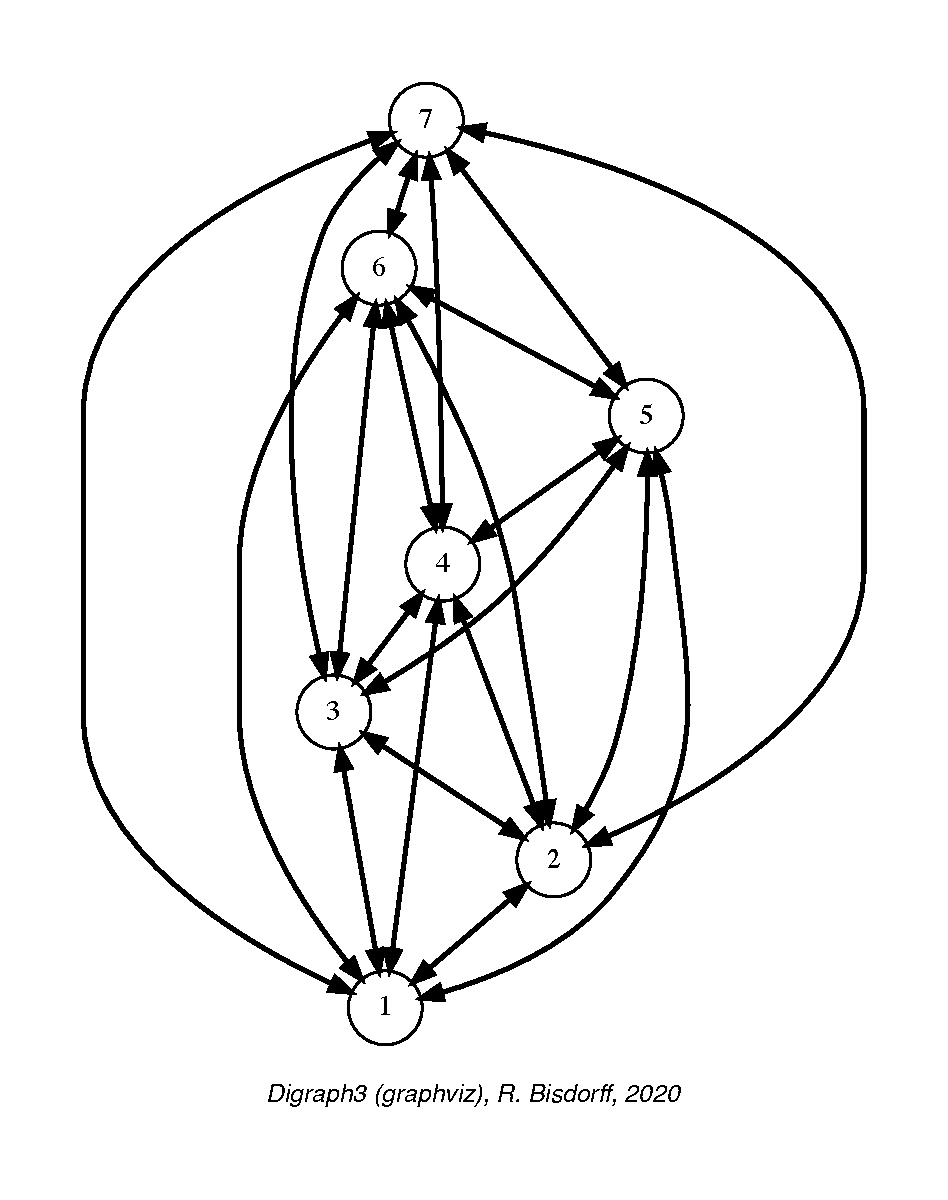
\includegraphics[width=6cm]{Figures/2-5-strongComponents.pdf}
\caption{Symmetric and transitive closure of the tutorial random valuation digraph $rdg$.}
\label{fig:2.5}       % Give a unique label
\end{figure}

The \texttt{closeSymmetric()}\index{closeSymmetric@\texttt{closeSymmetric()}} method (see List.~\vref{list:2.9} Line 2), of complexity $O(n^2)$ where $n$ denotes the digraph's order, changes, on the one hand, all single pairwise links it may detect into double links by operating a disjunction of the pairwise relations. On the other hand, the \texttt{closeTransitive()}\index{closeTransitive@\texttt{closeTransitive()}}  method (see Line 3), implements the \emph{Roy-Warshall} transitive closure algorithm of complexity $O(n^3)$ \index{Roy@\textsl{B. Roy}} \index{warshall@\textsl{S. Warshall}} (\citealp{ROY-1959} and \citealp{WAR-1962}).

The same \texttt{closeTransitive()} with a \texttt{Reverse = True} flag may be readily used for eliminating all transitive arcs from a transitive digraph instance. We make usage of this feature when drawing Hasse diagrams of \texttt{TransitiveDigraph}\index{TransitiveDigraph@\texttt{TransitiveDigraph} class} objects.

\section{Strong components}
\label{sec:2.8}

As the original digraph \texttt{rdg} was connected (see above the result of the showShort() command), both the symmetric and the transitive closures operated together, will necessarily produce a single strong component, i.e. a \textbf{complete} digraph. We may sometimes wish to collapse all strong components in a given digraph and construct the so \emph{collapsed} digraph. Using the \texttt{StrongComponentsCollapsedDigraph} constructor \index{StrongComponentsCollapsedDigraph@\texttt{StrongComponentsCollapsedDigraph} class} here will render a single hyper-node gathering all the original nodes (see Line 7 below).
\begin{lstlisting}[caption={Computing the strong components in a digraph},label=list:2.10]
>>> from digraphs import StrongComponentsCollapsedDigraph
>>> sc = StrongComponentsCollapsedDigraph(rdg)
>>> sc.showAll()
  *----- show detail -----*
   Digraph          : tutRandValDigraph_Scc
  *---- Actions ----*
    ['_7_1_2_6_5_3_4_']
  *---- Relation Table -----
      S     |  'Scc_1'	  
     -------|---------
     'Scc_1' |  0.00
  *---- strong Components ----*
   short 	 content
   'Scc_1' 	 '_7_1_2_6_5_3_4_'
  *---- Neighborhoods ----*
   Gamma     :
   'frozenset({'7','1','2','6','5','3','4'})':
                     in => set(), out => set()
   Not Gamma :
   'frozenset({'7','1','2','6','5','3','4'})':
                     in => set(), out => set()
\end{lstlisting}
  
\section{CSV storage}
\label{sec:2.9}

Sometimes it is required to exchange the graph valuation data in CSV format with a statistical package like \textbf{R}\footnote{\url{https://www.r-project.org/}}. For this purpose it is possible to export the digraph data into a CSV file. The valuation domain is hereby normalised by default to the range $[-1.0,1.0]$ and the diagonal is put by default to the minimal value $-1.0$.
\begin{lstlisting}
>>> rdg = Digraph('tutRandValDigraph')
>>> rdg.saveCSV('tutRandValDigraph')
  # content of file tutRandValDigraph.csv
  "d","1","2","3","4","5","6","7"
  "1",-1.0,0.48,-0.7,-0.86,-0.3,-0.38,-0.44
  "2",0.22,-1.0,0.38,-0.5,-0.8,0.54,-0.02
  "3",0.42,-0.08,-1.0,-0.7,0.56,-0.84,1.0
  "4",-0.44,0.4,0.62,-1.0,-0.04,-0.66,-0.76
  "5",-0.32,0.48,0.46,-0.64,-1.0,0.22,0.52
  "6",0.84,0.0,0.4,0.96,0.18,-1.0,0.22
  "7",-0.88,-0.72,-0.82,-0.52,0.84,-0.04,-1.0
\end{lstlisting}
  
It is possible to reload a \texttt{Digraph} instance from its previously saved CSV file content.
\begin{lstlisting} 
>>> from digraphs import CSVDigraph   
>>> rdgcsv = CSVDigraph('tutRandValDigraph')
>>> rdgcsv.showRelationTable(ReflexiveTerms=False)
    * ---- Relation Table -----
    r(xSy) |   '1'   '2'   '3'   '4'   '5'   '6'   '7'	  
    -------|------------------------------------------------------------
    '1'    |   -   -0.48  0.70  0.86  0.30  0.38  0.44	 
    '2'    | -0.22   -   -0.38  0.50  0.80 -0.54  0.02	 
    '3'    | -0.42  0.08   -    0.70 -0.56  0.84 -1.00	 
    '4'    |  0.44 -0.40 -0.62   -    0.04  0.66  0.76	 
    '5'    |  0.32 -0.48 -0.46  0.64   -   -0.22 -0.52	 
    '6'    | -0.84  0.00 -0.40 -0.96 -0.18   -   -0.22	 
    '7'    |  0.88  0.72  0.82  0.52 -0.84  0.04   -
\end{lstlisting}
  
It is as well possible to show a coloured version of the valued relation table in a system browser window tab (see Fig.~\vref{fig:2.5}).
\begin{lstlisting}
>>> rdgcsv.showHTMLRelationTable(tableTitle="Tutorial random digraph")
\end{lstlisting}
 \begin{figure}[ht]
\sidecaption[t]
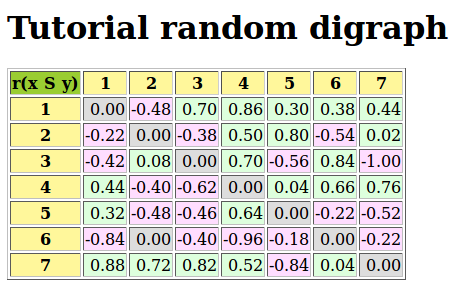
\includegraphics[width=7cm]{Figures/2-6-htmlTutorialDigraph.png}
\caption{The valued relation table shown in a browser window. Positive arcs are shown in green and negative arcs in red. Indeterminate --zero-valued-- links, like the reflexive diagonal ones or the link between node \texttt{'6'} and node \texttt{'2'}, are shown in gray}
\label{fig:2.6}       % Give a unique label
\end{figure}
 
\section{Complete, empty and indeterminate digraphs}
\label{sec:2.10}

Let us finally mention some special universal classes of digraphs that are readily available in the \texttt{digraphs} module\footnote{See \citealp{BIS-2021}}, like:
\begin{itemize}[nosep]
\item the \texttt{CompleteDigraph}\index{CompleteDigraph@\texttt{CompleteDigraph} class},
\item  the \texttt{EmptyDigraph}\index{EmptyDigraph@\texttt{EmptyDigraph} class} and
\item  the \texttt{IndeterminateDigraph}\index{IndeterminateDigraph@\texttt{IndeterminateDigraph} class} class,
\end{itemize}
who put all characteristic values respectively to the \emph{maximum}, the \emph{minimum} or the \emph{median} indeterminate characteristic value.
\begin{lstlisting}[caption={Complete, empty and indeterminate digraphs},label=list:2.11]
>>> from digraphs import CompleteDigraph,EmptyDigraph,\
...   			 IndeterminateDigraph
>>> # the empty digraph   
>>> e = EmptyDigraph(order=5)
>>> e.showRelationTable()
    * ---- Relation Table -----
      S   |    '1'    '2'    '3'    '4'	   '5'	  
    ---- -|-----------------------------------
    '1'   |  -1.00  -1.00  -1.00  -1.00	 -1.00	 
    '2'   |  -1.00  -1.00  -1.00  -1.00	 -1.00	 
    '3'   |  -1.00  -1.00  -1.00  -1.00	 -1.00	 
    '4'   |  -1.00  -1.00  -1.00  -1.00	 -1.00	 
    '5'   |  -1.00  -1.00  -1.00  -1.00	 -1.00
>>> e.showNeighborhoods() 
    Neighborhoods:
      Gamma     :
    '1': in => set(), out => set()
    '2': in => set(), out => set()
    '5': in => set(), out => set()
    '3': in => set(), out => set()
    '4': in => set(), out => set()
      Not Gamma :
    '1': in => {'2','4','5','3'}, out => {'2','4','5','3'}
    '2': in => {'1','4','5','3'}, out => {'1','4','5','3'}
    '5': in => {'1','2','4','3'}, out => {'1','2','4','3'}
    '3': in => {'1','2','4','5'}, out => {'1','2','4','5'}
    '4': in => {'1','2','5','3'}, out => {'1','2','5','3'}
>>> # the indeterminate digraph
>>> i = IndeterminateDigraph()
    * ---- Relation Table -----
      S   |   '1'   '2'	  '3'	'4'   '5'	  
    ------|------------------------------
    '1'   |  0.00  0.00	 0.00  0.00  0.00	 
    '2'   |  0.00  0.00	 0.00  0.00  0.00	 
    '3'   |  0.00  0.00	 0.00  0.00  0.00	 
    '4'   |  0.00  0.00	 0.00  0.00  0.00	 
    '5'   |  0.00  0.00	 0.00  0.00  0.00	 
>>> i.showNeighborhoods()
    Neighborhoods:
      Gamma     :
    '1': in => set(), out => set()
    '2': in => set(), out => set()
    '5': in => set(), out => set()
    '3': in => set(), out => set()
    '4': in => set(), out => set()
      Not Gamma :
    '1': in => set(), out => set()
    '2': in => set(), out => set()
    '5': in => set(), out => set()
    '3': in => set(), out => set()
    '4': in => set(), out => set()
\end{lstlisting}

Mind the subtle difference between the neighbourhoods of an \emph{empty} and the neighbourhoods of an \emph{indeterminate} digraph instance. In the first kind, the neighbourhoods are known to be completely \emph{empty}  (see List.~\vref{list:2.11} Lines 22-27) whereas, in the latter, \emph{nothing is known} about the actual neighbourhoods of the nodes  (see Lines 46-51). These two cases illustrate why in the case of \emph{bipolar-valued} digraphs, we may sometimes need both a \texttt{gamma} \textbf{and} a \texttt{notGamma} attribute.

\vspace{1cm}
In the following Chapter~\ref{sec:3}  we introduce the main formal object of this book, namely \emph{bipolar-valued outranking} digraphs.

%%%%%%%%%%%%%%%%%%%%%%%%%%%%%%%%%%%%
\phantomsection
\addcontentsline{toc}{section}{Notes}
\section*{Notes}

It is \emph{D. Bouyssou} \index{Bouyssou@\emph{D. Bouyssou}} who first suggested us end of the nineties, when we started to work in Prolog on the computation of digraph kernels with finite domain constraint solvers, that the $50\%$ criteria significance majority was a special value to be carefully taken into account. The converging solution vectors of the fixpoint kernel equations confirmed this special status of the $50\%$ majority (see Chap.~\ref{sec:17}). These early insights led to the seminal articles on bipolar-valued epistemic logic where we introduced split truth/falseness semantics for a multi-valued logical processing of fuzzy preference modelling \citep{BIS-2000,BIS-2002}. The characteristic valuation domain remained however the classical fuzzy $[0.0;1.0]$ valuation domain.

It is only in 2004, when we succeeded in assessing the stability of the outranking digraph when solely ordinal criteria significance weights are given, that it became clear and evident for us that the characteristic valuation domain had to be shifted to a bipolar $[-1.0;+1.0]$-valued domain \citep{BIS-2004a}. In this bipolar valuation domain, the $50\%$ majority thershold corresponds now to the median $0.0$ value, characterising with the correct zero value an epistemic indetermination --no knowledge-- situation. Furthermore, identifying truth and falseness by the sign of the characteristic values revealed itself to be very efficient not only from a computational point of view, but also from scientific and semiotical perspectives. A positive (resp. negative) characteristic value now attest a logically valid (resp. invalid) statement and a negative affirmation now corresponds to a positive refutation. Furthermore, the median zero value gives way to efficiently handling partial digraphs --like the border or the assymetric part of a digraph-- and, even more important from a practical decision making point of view, any missing data.

The bipolar $[-1.0;+1.0]$-valued characteritisc domain opened so the way to important new operations and concepts, like the disjunctive epistemic fusion operation seen in Section~\vref{sec:2.5} that confers the outranking digraph a logically and epistemically sound definition \citep{BIS-2013}. \Kendall 's ordinal correlation index could be extended to a bipolar-valued relational equivalence index between digraphs \citep{BIS-2012a}. Making usage of the bipolar-valued Gaussian error function naturally led to defining a bipolar-valued likelihood function, where a positive (resp. negative) value gives the likelihood of an affirmation (resp. a refutation) \citep{BIS-2014}.      

%%%%%%% The chapter bibliography
%\normallatexbib
%\clearpage
%\phantomsection
%\addcontentsline{toc}{section}{Chapter Bibliograhy}
\bibliographystyle{spbasic}
%\typeout{}
\bibliography{03-backMatters/reference}
%\chapter{Working with bipolar-valued digraphs}
\label{sec:2}

\abstract*{ The chapter introduces bipolar-valued digraphs, the fondamental root type of all the specialised digraphs implemented in the \Digraph modules. With the help of a randomly valued digraph, we illustrate some basic digraph manipulation methods, like drawing the digraph, dividing the digraph into its asymmetric and symmetric parts, separating the border from the inner part, computing associated dual, converse and codual digraphs, and operating symmetric and transitive closures.}

\abstract{ The chapter introduces bipolar-valued digraphs, the fondamental root type of all the specialised digraphs implemented in the \Digraph modules. With the help of a randomly valued digraph, we illustrate some basic digraph manipulation methods, like drawing the digraph, dividing the digraph into its asymmetric and symmetric parts, separating the border from the inner part, computing associated dual, converse and codual digraphs, and operating symmetric and transitive closures.}

\section{Random bipolar-valued digraphs}

In Listing~\vref{list:2.1}, we generate a uniformly random $[-1.0; +1.0]$-valued digraph of order 7, denoted \texttt{rdg} and modelling, for instance, a binary relation $S(x,y)$ defined on the set of nodes of \texttt{rdg}. For this purpose, the \Digraph resources provide in the \texttt{randomDigraphs}\index{randomDigraphs@\texttt{randomDigraphs} module} module a specific \texttt{RandomValuationDigraph}\index{RandomValuationDigraph@\texttt{RandomValuationDigraph} class} class \citep{BIS-2021b}.
\begin{lstlisting}[caption={Random bipolar-valued digraph instance},label=list:2.1]
>>> from randomDigraphs import RandomValuationDigraph
>>> rdg = RandomValuationDigraph(order=7)
>>> rdg.save('tutRandValDigraph')
>>> from digraphs import Digraph
>>> rdg = Digraph('tutRandValDigraph')
>>> rdg
  *------- Digraph instance description ------*
   Instance class      : Digraph
   Instance name       : tutRandValDigraph
   Digraph Order       : 7
   Digraph Size        : 22
   Valuation domain    : [-1.00;1.00]
   Determinateness (%) : 75.24
   Attributes          : ['name','actions','order',
                          'valuationdomain','relation',
                          'gamma','notGamma']
\end{lstlisting}   

With the \texttt{save()} \index{save@\texttt{save()}} method (see Line 3) we keep for future use a backup version of \texttt{rdg} which is saved into a file named \texttt{tutRandValDigraph.py} in the current working directory. The genuine \texttt{Digraph} class constructor may restore the \texttt{rdg} object from the stored file (Lines 4-5). We may easily inspect the content of \texttt{rdg} (Line 6). The digraph size 22 indicates the number of positively valued arcs. The valuation domain is uniformly distributed in the interval $[-1.0; 1.0]$ and the mean absolute arc valuation is $(0.7524 \times 2)\, -\, 1.0 \;=\; 0.5048$ (Line 13).

As mentioned in the previous Chapter~\ref{sec:1}, all objects of \texttt{Digraph} type contain at least the list of attributes shown here in Lines 14-16: --a \texttt{name} (string), --a dictionary of \texttt{actions} (digraph nodes), --an \texttt{order} (integer) attribute containing the number of actions, --a \texttt{valuationdomain} dictionary, --a double dictionary \texttt{relation} representing the adjacency table of the digraph relation, --a \texttt{gamma} and --a {\tt notGamma} dictionary containing the direct neighbourhood of each action.

The \texttt{Digraph} class provides some generic \texttt{show...()} methods for exploring the content of a given \texttt{ Digraph} object, like the \texttt{showRelationTable()}\index{showRelationTable@\texttt{showRelationTable()}}, the \texttt{showComponents()}\index{showComponents@\texttt{showComponents()}} and the \texttt{showNeighborhoods()}\index{showNeighborhoods@\texttt{showNeighborhoods()}} methods.
\begin{lstlisting}[caption={Example of random valuation digraph},label=list:2.2]
>>> rdg.showRelationTable()
  * ---- Relation Table -----
   r(xSy) |  '1'    '2'   '3'  '4'   '5'    '6'  '7'	  
   -------|-------------------------------------------
    '1'   |  0.00 -0.48  0.70  0.86  0.30  0.38  0.44	 
    '2'   | -0.22  0.00 -0.38  0.50  0.80 -0.54  0.02	 
    '3'   | -0.42  0.08  0.00  0.70 -0.56  0.84 -1.00	 
    '4'   |  0.44 -0.40 -0.62  0.00  0.04  0.66  0.76	 
    '5'   |  0.32 -0.48 -0.46  0.64  0.00 -0.22 -0.52	 
    '6'   | -0.84  0.00 -0.40 -0.96 -0.18  0.00 -0.22	 
    '7'   |  0.88  0.72  0.82  0.52 -0.84  0.04  0.00
>>> rdg.showComponents()
  *--- Connected Components ---*
  1: ['1', '2', '3', '4', '5', '6', '7']
>>> rdg.showNeighborhoods()
  *---- Neighborhoods ------*
     Gamma:
     '1': in => {'5','7','4'}, out => {'5','7','6','3','4'}
     '2': in => {'7','3'},out => {'5','7','4'}
     '3': in => {'7','1'}, out => {'6','2','4'}
     '4': in => {'5','7','1','2','3'}, out => {'5','7','1','6'}
     '5': in => {'1','2','4'}, out => {'1','4'}
     '6': in => {'7','1','3','4'}, out => set()
     '7': in => {'1','2','4'}, out => {'1','2','3','4','6'}
     Not Gamma:
     '1': in => {'6','2','3'}, out => {'2'}
     '2': in => {'5','1','4'}, out => {'1','6','3'}
     '3': in => {'5','6','2','4'}, out => {'5','7','1'}
     '4': in => {'6'}, out => {'2','3'}
     '5': in => {'7','6','3'}, out => {'7','6','2','3'}
     '6': in => {'5','2'}, out => {'5','7','1','3','4'}
     '7': in => {'5','6','3'}, out => {'5'}
\end{lstlisting}   

Mind that some \texttt{Digraph} class methods will ignore the \emph{reflexive} links by considering that they are \emph{indeterminate}, i.e. the characteristic value $r(x\,S\,x)$ for all action $x$ is set to the \emph{median}, i.e. \emph{indeterminate} value $0.0$ in this case (see Listing~\vref{list:2.2} Lines 5-11 and \citet{BIS-2004a}).

\section{Graphviz drawings}
\label{sec:2.2}

An even better insight into the \texttt{Digraph} object \texttt{rdg} is given by looking at its \href{https://graphviz.org/}{graphviz} drawing \citep{graphviz}\footnote{The \texttt{exportGraphViz()} method is depending on drawing tools from the graphviz software (https://graphviz.org/). On Linux Ubuntu or Debian you may try \texttt{sudo apt-get install graphviz} to install them. There are ready \emph{dmg} installers for Mac OSX.}\index{graphviz}.
\begin{lstlisting}
>>> rdg.exportGraphViz('tutRandValDigraph')
 *---- exporting a dot file for GraphViz tools ------*
  Exporting to tutRandValDigraph.dot
  dot -Grankdir=BT -Tpng tutRandValDigraph.dot\
                           -o tutRandValDigraph.png
\end{lstlisting}
\begin{figure}[ht]
\sidecaption[t]
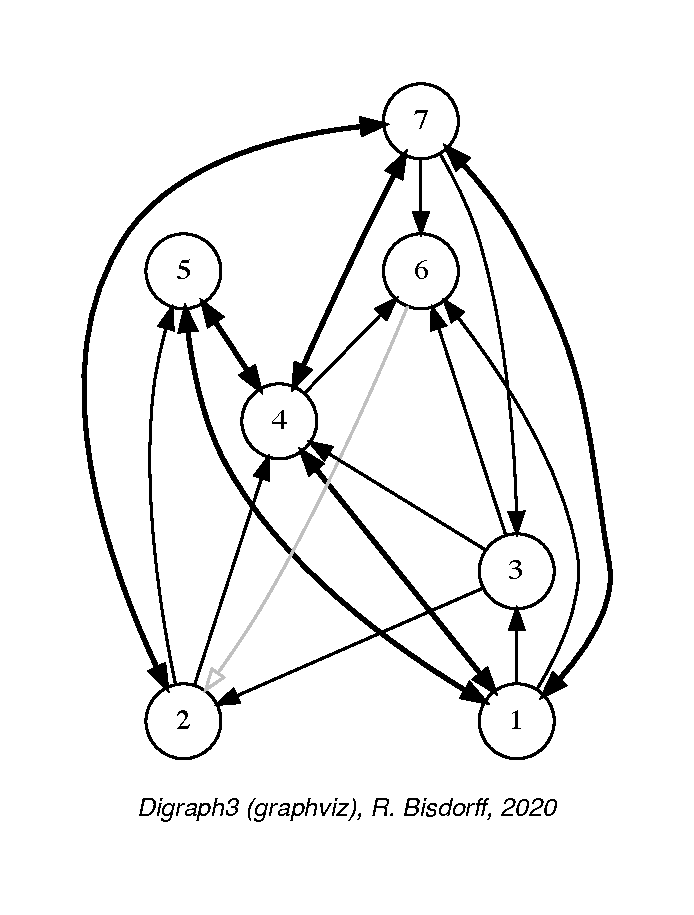
\includegraphics[width=6cm]{Figures/2-1-tutRandValDigraph.pdf}
\caption{\emph{The tutorial random valuation digraph}. Double links are drawn in bold black with an arrowhead at each end, whereas single asymmetric links are drawn in black with an arrowhead showing the direction of the link. Notice the undetermined relational situation ($r(6\,S\,2) = 0.00$) observed between nodes '6' and '2'. The corresponding link is marked in gray with an open arrowhead in the drawing}
\label{fig:2.1}       % Give a unique label
\end{figure}
  
\section{Asymmetric and symmetric parts}
\label{sec:2.3}

We may now extract both the \emph{}\emph{symmetric} as well as the \emph{asymmetric} part of digraph \texttt{rdg} with the help of two corresponding constructors (see List.~\vref{list:2.3}) \index{AsymmetricPartialDigraph@\texttt{AsymmetricPartialDigraph} class}\index{SymmetricPartialDigraph@\texttt{SymmetricPartialDigraph} class}.
\begin{lstlisting}[caption={Computing asymmetric and symmetric Parts},label=list:2.3]
>>> from digraphs import AsymmetricPartialDigraph,\
...                      SymmetricPartialDigraph
>>> asymDg = AsymmetricPartialDigraph(rdg)
>>> asymDg.exportGraphViz()
>>> symDg = SymmetricPartialDigraph(rdg)
>>> symDg.exportGraphViz()
\end{lstlisting}
\begin{figure}[ht]
  % \sidecaption
  Asymmetric Part \hfill Symmetric Part \\
  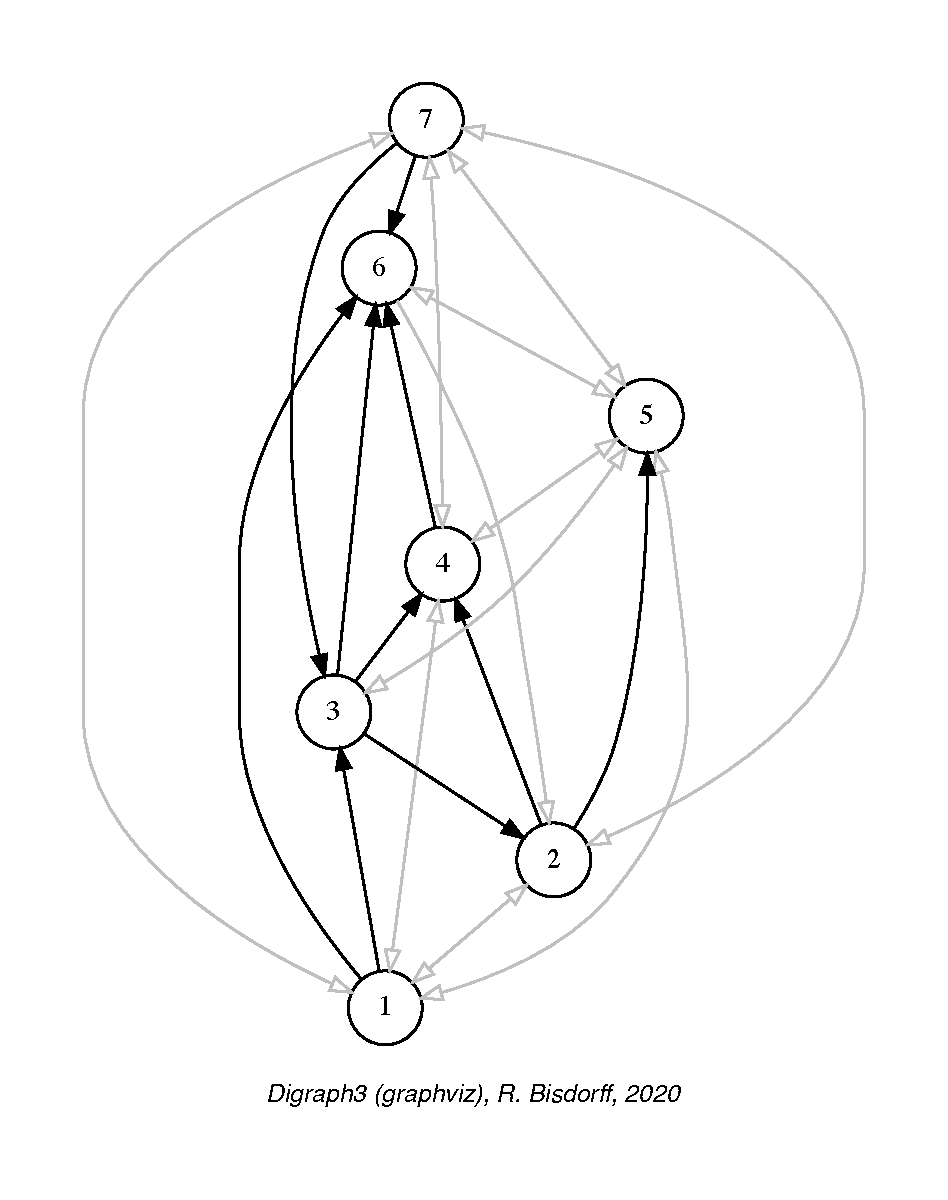
\includegraphics[height=6cm]{Figures/2-2-asymmetricPart.pdf}\hfill
  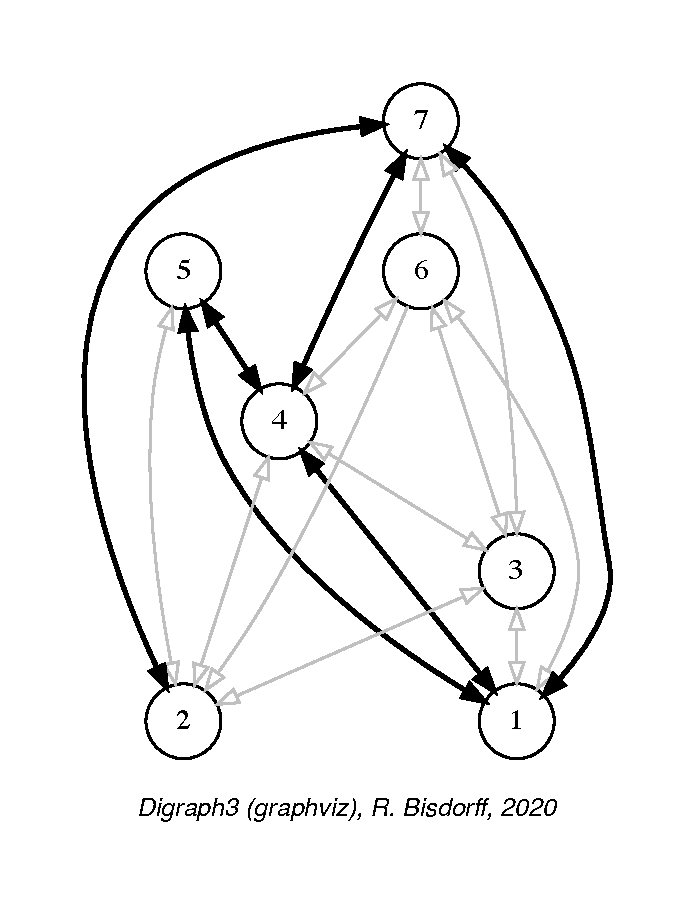
\includegraphics[height=6cm]{Figures/2-2-symmetricPart.pdf}\hfill
\caption{Asymmetric and symmetric part of the tutorial random valuation digraph}
\label{fig:2.2}       % Give a unique label
\end{figure}

The constructor of the partial objects \texttt{asymDg} and \texttt{symDg} puts to the indeterminate characteristic value all non-asymmetric, respectively non-symmetric links between nodes (see Fig.~\vref{fig:2.2}).

Here below, for illustration the source code of the \texttt{ relation} constructor of the \texttt{AsymmetricPartialDigraph} class.
\begin{lstlisting}[caption={Computing the asymmetric part of a bipolar-valued relation},label=list:2.4,basicstyle=\ttfamily\scriptsize]
def _constructRelation(self):
    actions = self.actions
    Min = self.valuationdomain['min']
    Max = self.valuationdomain['max']
    Med = self.valuationdomain['med']
    relationIn = self.relation
    relationOut = {}
    for a in actions:
	relationOut[a] = {}
	for b in actions:
	    if a != b:
                if relationIn[a][b] >= Med and relationIn[b][a] <= Med:
		    relationOut[a][b] = relationIn[a][b]
		elif relationIn[a][b] <= Med and relationIn[b][a] >= Med:
		    relationOut[a][b] = relationIn[a][b]
		else:
		    relationOut[a][b] = Med
	    else: # reflexive links are ignored
		relationOut[a][b] = Med
    return relationOut
\end{lstlisting}

\section{Border and inner parts}
\label{sec:2.4}

We may also extract the \emph{border} --the part of a digraph induced by the union of its initial and terminal prekernels (see Chap.~\ref{sec:17})--  as well as, the \emph{inner part} --the complement of the border-- with the help of two corresponding class constructors: \texttt{GraphBorder}\index{GraphBorder@\texttt{GraphBorder} class} and \texttt{GraphInner}\index{GraphInner@\texttt{GraphInner} class} (see Fig.~\vref{fig:2.3}).

\begin{figure}[ht]
%\sidecaption
  Border Part \hfill Inner Part \\
  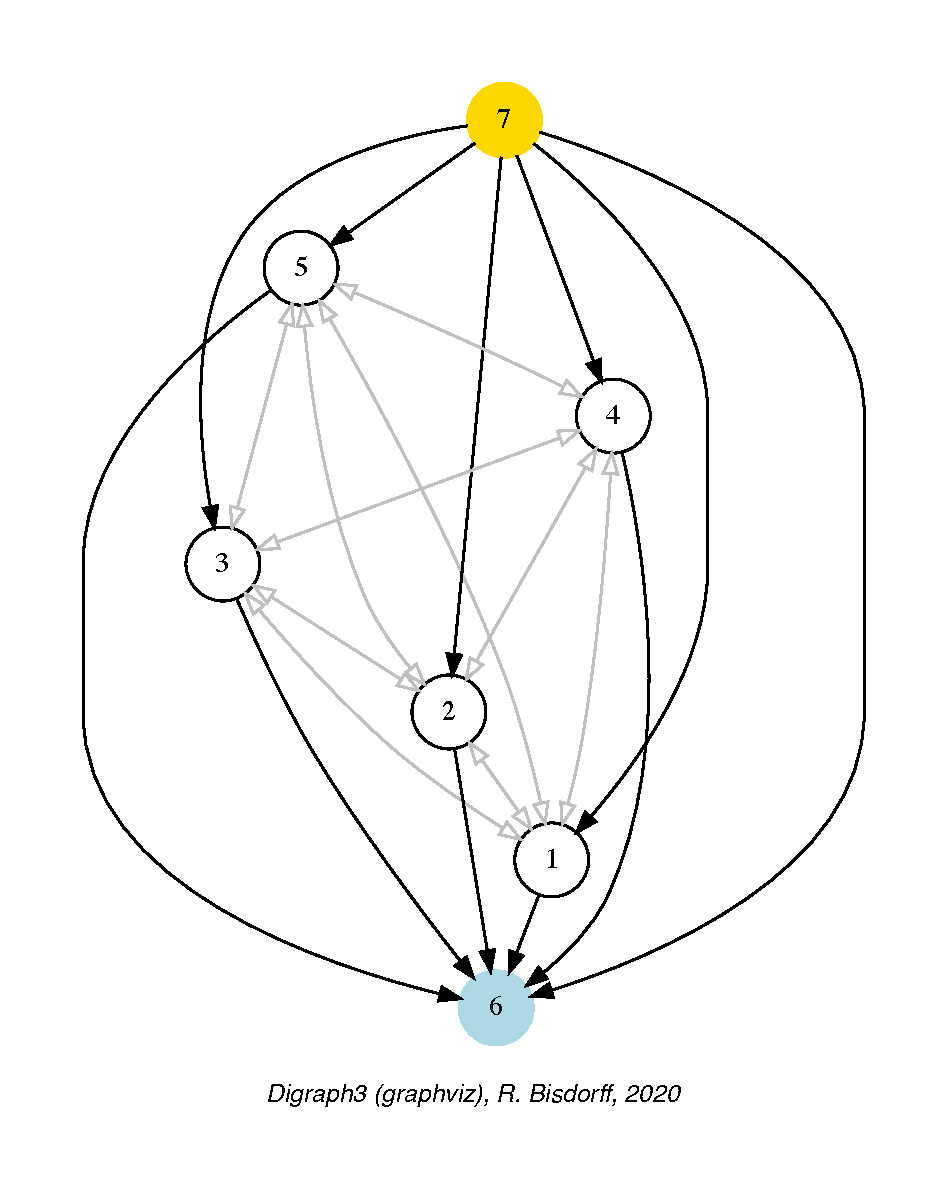
\includegraphics[height=6cm]{Figures/2-3-linearOrderBorder.pdf}\hfill
  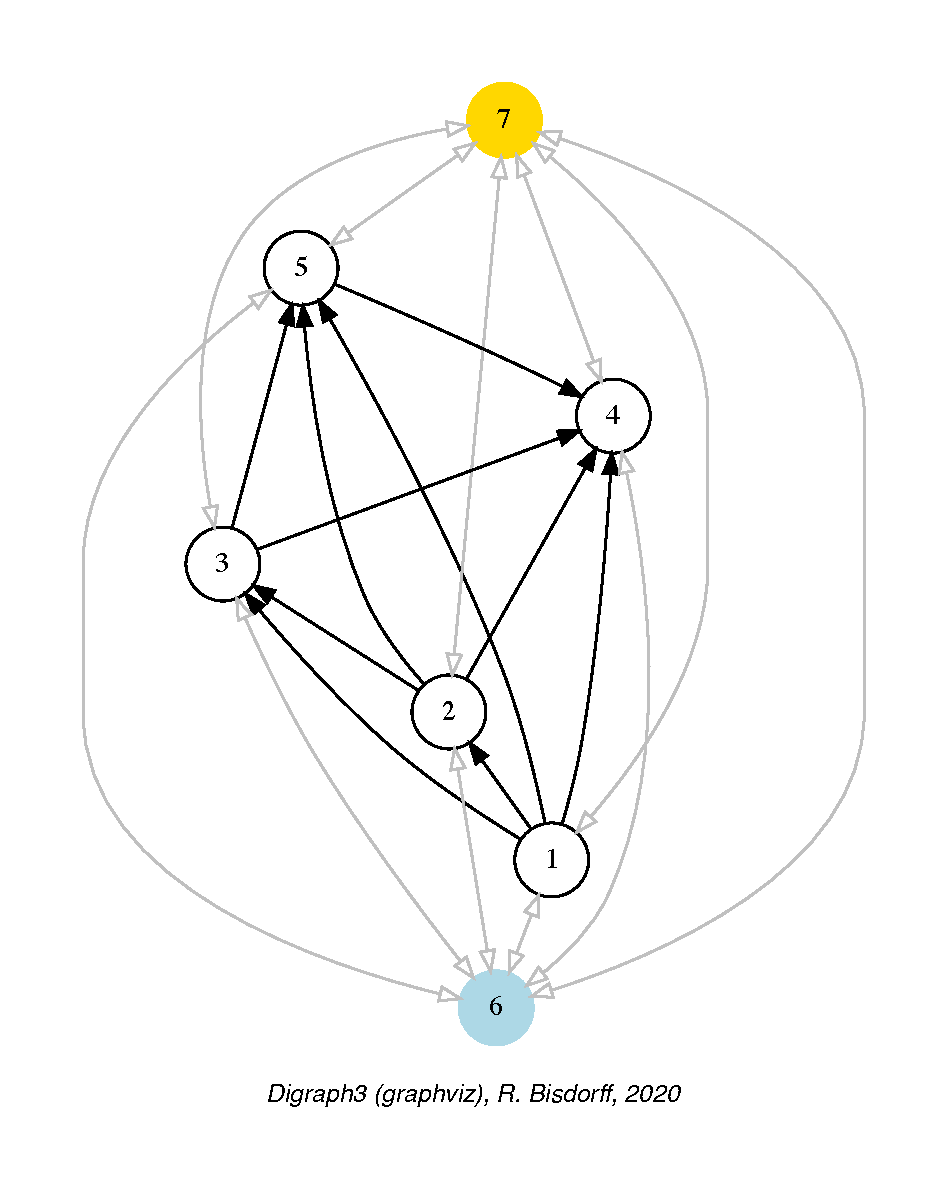
\includegraphics[height=6cm]{Figures/2-3-linearOrderInner.pdf}\hfill
\caption{\emph{Border} and \emph{inner} part of a linear order oriented by \emph{terminal} and \emph{initial} kernels.}
\label{fig:2.3}       % Give a unique label
\end{figure}
Let us illustrate the digraph border and inner parts on a linear ordering obtained from the tutorial random valuation digraph \texttt{rdg}  with the \NetFlows ranking rule  (see Sec.~\ref{sec:8.3}).  
\begin{lstlisting}[caption={Border and inner part of a linear order},label=list:2.5]
>>> from digraphs import GraphBorder, GraphInner
>>> from linearOrders import NetFlowsOrder
>>> nf = NetFlowsOrder(rdg)
>>> nf.netFlowsOrder
   ['6', '4', '5', '3', '2', '1', '7']
>>> bnf = GraphBorder(nf)
>>> bnf.exportGraphViz(lastChoice=['6'],firstChoice=['7'])
>>> inf = GraphInner(nf)
>>> inf.exportGraphViz(lastChoice=['6'],firstChoice=['7'])
\end{lstlisting}
We may orient the \texttt{graphviz} drawings in Figure~\vref{fig:2.3}  with the terminal node 6 (\texttt{lastChoice} parameter) and initial node 7 (\texttt{firstChoice} parameter) (see List.~\vref{list:2.5} Lines 7 and 9).

The constructor of the partial digraphs \texttt{bnf} and \texttt{inf}  (see Lines 3 and 6) puts to the \emph{indeterminate} characteristic value all links not in the \emph{border}, respectively \emph{not} in the \emph{inner} part (see Fig.~\vref{fig:2.3}). Being much {\em denser\/} than a linear order, the actual inner part of our tutorial random valuation digraph \texttt{rdg} is reduced to a single arc between nodes 3 and 4 (see Fig.~\vref{fig:2.4}). Indeed, a complete digraph on the limit has no inner part (privacy!) at all, whereas empty and indeterminate digraphs admit both, an empty border and an empty inner part.
\begin{figure}[h]
%\sidecaption
  Border Part \hfill Inner Part \\
  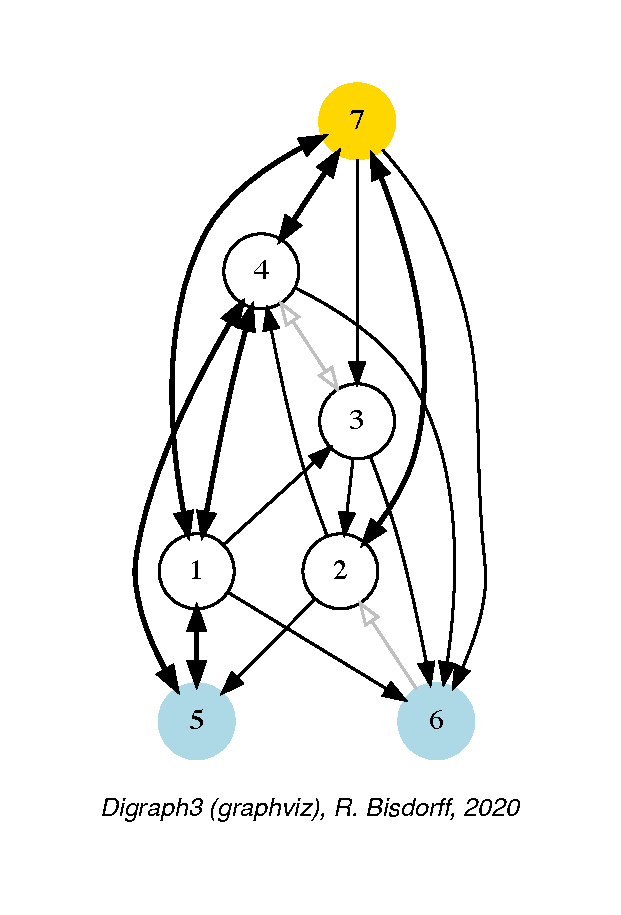
\includegraphics[height=6cm]{Figures/2-4-tutRandValDigraph_border.pdf}\hfill
  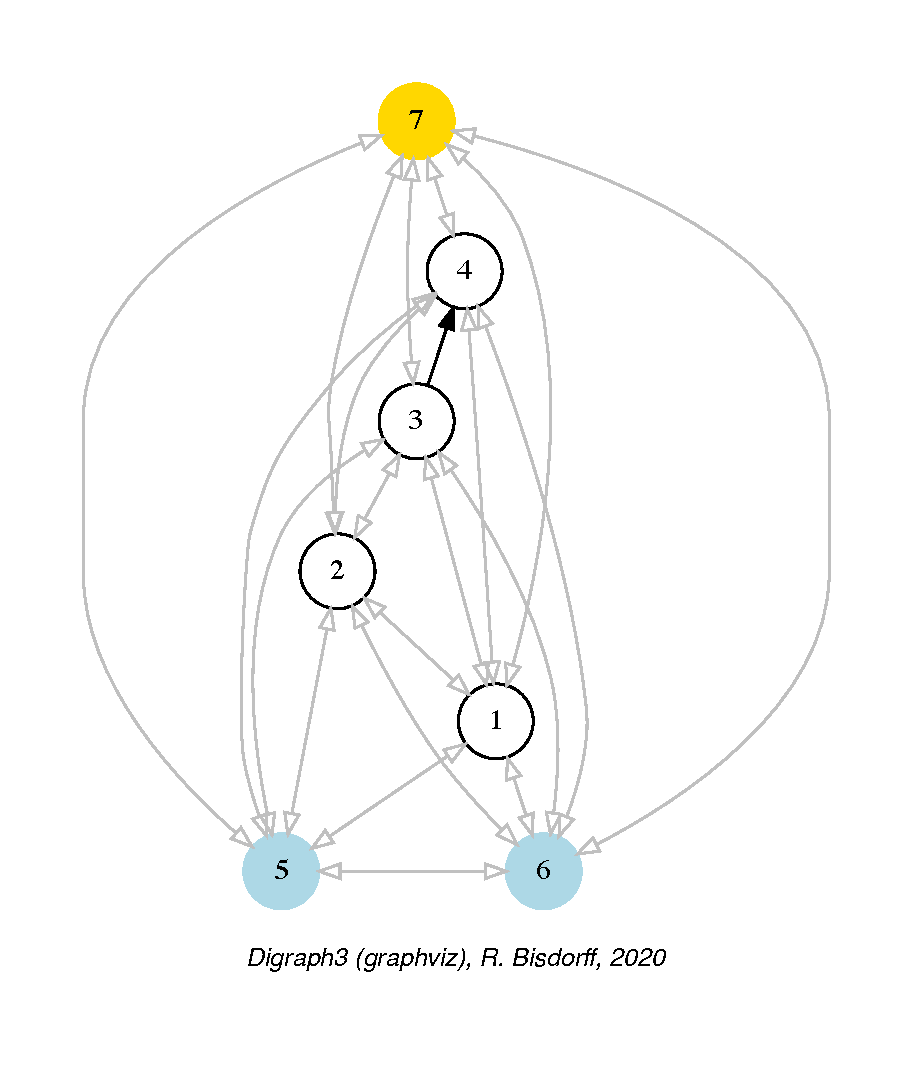
\includegraphics[height=6cm]{Figures/2-4-tutRandValDigraph_inner.pdf}\hfill
\caption{Border and inner part of the tutorial random valuation digraph \texttt{rdg}}
\label{fig:2.4}       % Give a unique label
\end{figure}

\section{Fusion by epistemic disjunction}
\label{sec:2.5}

We may recover object \texttt{rdg} from both partial objects \texttt{asymDg} and \texttt{symDg}, or as well from the border \texttt{bg} and the inner part \texttt{ig}, with a \emph{bipolar fusion} operator, also called \emph{epistemic disjunction}, available via the \texttt{FusionDigraph}\index{FusionDigraph@\texttt{FusionDigraph} class} class. 
\begin{lstlisting}[caption={Epistemic fusion of partial diagraphs},label=list:2.6]
>>> from digraphs import FusionDigraph
>>> fusDg = FusionDigraph(asymDg,symDg,operator='o-max')
>>> # fusDg = FusionDigraph(bg,ig,operator='o-max')
>>> fusDg.showRelationTable()
  * ---- Relation Table -----
   r(xSy) |  '1'    '2'   '3'  '4'   '5'    '6'  '7'	  
   -------|------------------------------------------
    '1'   |  0.00 -0.48  0.70  0.86  0.30  0.38  0.44	 
    '2'   | -0.22  0.00 -0.38  0.50  0.80 -0.54  0.02	 
    '3'   | -0.42  0.08  0.00  0.70 -0.56  0.84 -1.00	 
    '4'   |  0.44 -0.40 -0.62  0.00  0.04  0.66  0.76	 
    '5'   |  0.32 -0.48 -0.46  0.64  0.00 -0.22 -0.52	 
    '6'   | -0.84  0.00 -0.40 -0.96 -0.18  0.00 -0.22	 
    '7'   |  0.88  0.72  0.82  0.52 -0.84  0.04  0.00
\end{lstlisting}

The epistemic fusion operator \texttt{o-max} (see List.~\vref{list:2.6} Line 2) is defined as follows:
\begin{definition}[Disjunctive epistemic fusion operator \texttt{o-max}]\label{def:disjunctiveFusion}

\noindent Let $r$ and $r'$ characterise two bipolar-valued epistemic situations:
\begin{itemize}[leftmargin=0.5cm,rightmargin=0.5cm,nosep]
\item \texttt{o-max}$(r, r')$ = $\max(r, r' )$ when both $r$ and $r'$ are more or less valid or indeterminate;
\item \texttt{o-max}$(r, r')$ = $\min(r, r' )$ when both $r$ and $r'$ are more or less invalid or indeterminate;
\item \texttt{o-max}$(r, r')$ = $0.0$, i.e. indeterminate otherwise.
\end{itemize}
\end{definition}

Mind that the \texttt{o-max} operator, like a mean operator, is \emph{not associative} when more than 2 operands are given. In order to make the \texttt{o-max} fusion univocal, the following rule is applied: --first, all positive and negative terms are separately aggregated, --then the \texttt{o-max} fusion is applied on both aggregates.

\section{Dual, converse and codual digraphs}
\label{sec:2.6}

We may as readily compute the \emph{dual}\index{DualDigraph@\texttt{DualDigraph} class} (negated relation \footnote{Not to be confused with the dual graph of a plane graph $g$ that has a vertex for each face of $g$. Here we mean the \emph{less than} (strict converse) relation corresponding to a \emph{greater or equal} relation, or the \emph{less than or equal} relation corresponding to a (strict) \emph{better than} relation.}), the \emph{converse}\index{ConverseDigraph@\texttt{ConverseDigraph} class} (transposed relation) and the \emph{codual}\index{CoDualDigraph@\texttt{CoDualDigraph} class} (transposed and negated relation) of the digraph instance \texttt{rdg}. 
\begin{lstlisting}[caption={Computing associated dual, converse and codual digraphs},label=list:2.7]
>>> from digraphs import\
...          DualDigraph, ConverseDigraph, CoDualDigraph
>>> # dual of rdg
>>> ddg = DualDigraph(rdg)
>>> ddg.showRelationTable()
    -r(xSy) |  '1'    '2'   '3'  '4'   '5'    '6'  '7'	  
    --------|------------------------------------------
    '1 '    |  0.00  0.48 -0.70 -0.86 -0.30 -0.38 -0.44	 
    '2'     |  0.22  0.00  0.38 -0.50  0.80  0.54 -0.02	 
    '3'     |  0.42  0.08  0.00 -0.70  0.56 -0.84  1.00	 
    '4'     | -0.44  0.40  0.62  0.00 -0.04 -0.66 -0.76	 
    '5'     | -0.32  0.48  0.46 -0.64  0.00  0.22  0.52	 
    '6'     |  0.84  0.00  0.40  0.96  0.18  0.00  0.22	 
    '7'     |  0.88 -0.72 -0.82 -0.52  0.84 -0.04  0.00
>>> # converse of rdg
>>> cdg = ConverseDigraph(rdg)
>>> cdg.showRelationTable()
    * ---- Relation Table -----
     r(ySx) |  '1'    '2'   '3'   '4'   '5'   '6'   '7'	  
    --------|------------------------------------------
    '1'     |  0.00 -0.22 -0.42  0.44  0.32 -0.84  0.88	 
    '2'     | -0.48  0.00  0.08 -0.40 -0.48  0.00  0.72	 
    '3'     |  0.70 -0.38  0.00 -0.62 -0.46 -0.40  0.82	 
    '4'     |  0.86  0.50  0.70  0.00  0.64 -0.96  0.52	 
    '5'     |  0.30  0.80 -0.56  0.04  0.00 -0.18 -0.84	 
    '6'     |  0.38 -0.54  0.84  0.66 -0.22  0.00  0.04	 
    '7'     |  0.44  0.02 -1.00  0.76 -0.52 -0.22  0.00	 
>>> # codual of rdg
>>> cddg = CoDualDigraph(rdg)
>>> cddg.showRelationTable()
    * ---- Relation Table -----
    -r(ySx) |  '1'    '2'   '3'   '4'   '5'   '6'   '7'	    
    --------|------------------------------------------
    '1'     |  0.00  0.22  0.42 -0.44 -0.32  0.84 -0.88	 
    '2'     |  0.48  0.00 -0.08  0.40  0.48  0.00 -0.72	 
    '3'     | -0.70  0.38  0.00  0.62  0.46  0.40 -0.82	 
    '4'     | -0.86 -0.50 -0.70  0.00 -0.64  0.96 -0.52	 
    '5'     | -0.30 -0.80  0.56 -0.04  0.00  0.18  0.84	 
    '6'     | -0.38  0.54 -0.84 -0.66  0.22  0.00 -0.04	 
    '7'     | -0.44 -0.02  1.00 -0.76  0.52  0.22  0.00	 
\end{lstlisting}

Computing the \emph{dual}, respectively the \emph{converse} of a digraph, may also be done with prefixing the \texttt{\_\_neg\_\_} ($-$) or the \texttt{\_\_invert\_\_} ($\sim$) operator. The \emph{codual} of a \texttt{Digraph} object may, hence, as well be computed with a \emph{composition} (in either order) of both operations.
\begin{lstlisting}[caption={Computing the dual, the converse and the codual of a digraph},label=list:2.8]
>>> ddg = -rdg   # dual of rdg
>>> cdg = ~rdg   # converse of rdg
>>> cddg = ~(-rdg) # = -(~(rdg) codual of rdg
>>> (-(~rdg)).showRelationTable()
  * ---- Relation Table -----
   -r(ySx) |  '1'    '2'   '3'   '4'   '5'   '6'   '7'	    
   --------|------------------------------------------
   '1'     |  0.00  0.22  0.42 -0.44 -0.32  0.84 -0.88	 
   '2'     |  0.48  0.00 -0.08  0.40  0.48  0.00 -0.72	 
   '3'     | -0.70  0.38  0.00  0.62  0.46  0.40 -0.82	 
   '4'     | -0.86 -0.50 -0.70  0.00 -0.64  0.96 -0.52	 
   '5'     | -0.30 -0.80  0.56 -0.04  0.00  0.18  0.84	 
   '6'     | -0.38  0.54 -0.84 -0.66  0.22  0.00 -0.04	 
   '7'     | -0.44 -0.02  1.00 -0.76  0.52  0.22  0.00	 
\end{lstlisting}
  
\section{Symmetric and transitive closures}
\label{sec:2.7}

Symmetric and transitive closures, by default in-site methods, are also available (see Fig.~\vref{fig:2.5})\index{closeSymmetric@\texttt{closeSymmetric()}}\index{closeTransitive@\texttt{closeTransitive()}}. Note that it is a good idea, before going ahead with these in-site operations, who irreversibly modify the original \texttt{rdg} object, to previously make a backup version of \texttt{rdg}. The simplest storage method, always provided by the generic \texttt{Digraph.save()} method, writes out in a named file the python content of the Digraph object in string representation (see Sec.~\vref{sec:1.3}).
\begin{lstlisting}[caption={Symmeric and transitive closures},label=list:2.9]
>>> rdg.save('tutRandValDigraph')
>>> rdg.closeSymmetric(InSite=True)
>>> rdg.closeTransitive(InSite=True)
>>> rdg.exportGraphViz('strongComponents')
\end{lstlisting}
\begin{figure}[h]
\sidecaption[t]
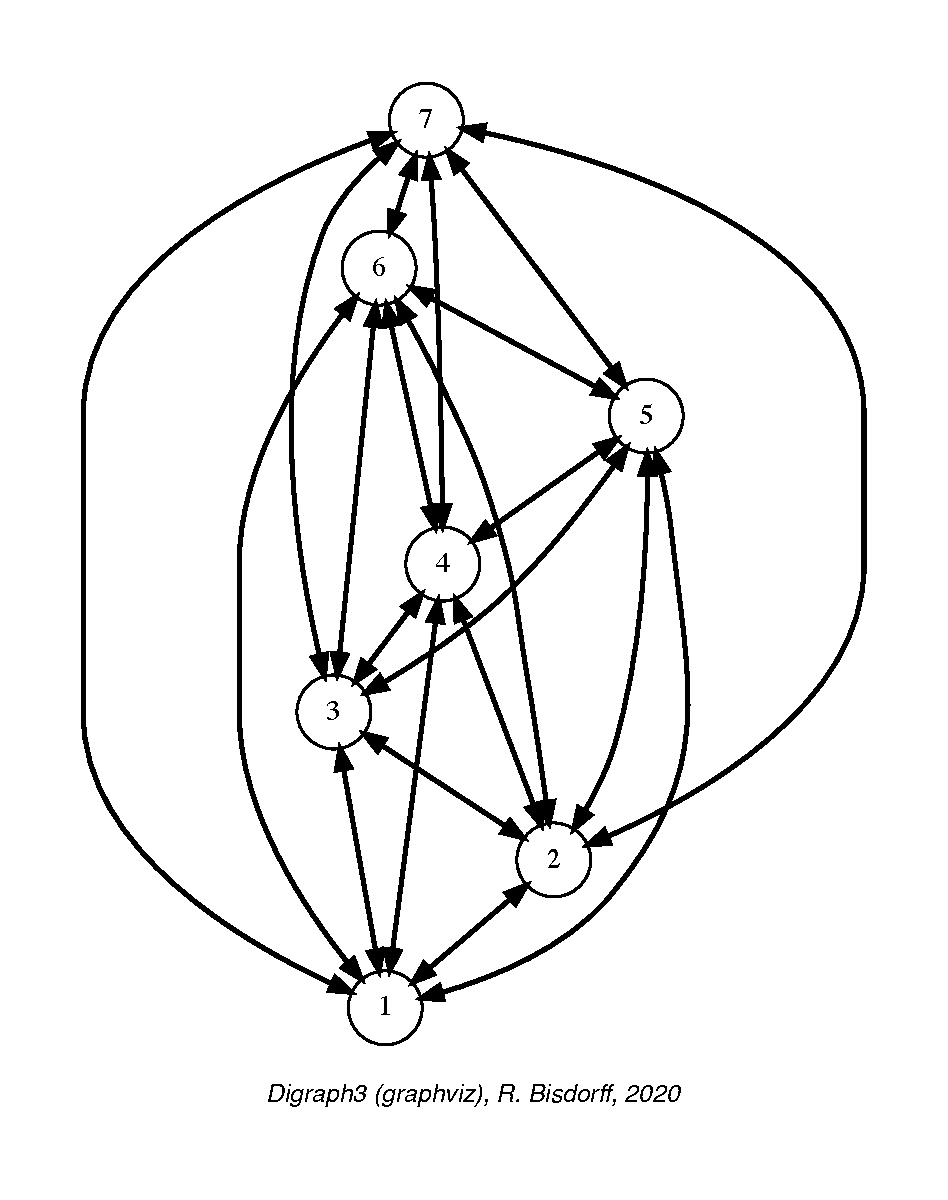
\includegraphics[width=6cm]{Figures/2-5-strongComponents.pdf}
\caption{Symmetric and transitive closure of the tutorial random valuation digraph $rdg$.}
\label{fig:2.5}       % Give a unique label
\end{figure}

The \texttt{closeSymmetric()}\index{closeSymmetric@\texttt{closeSymmetric()}} method (see List.~\vref{list:2.9} Line 2), of complexity $O(n^2)$ where $n$ denotes the digraph's order, changes, on the one hand, all single pairwise links it may detect into double links by operating a disjunction of the pairwise relations. On the other hand, the \texttt{closeTransitive()}\index{closeTransitive@\texttt{closeTransitive()}}  method (see Line 3), implements the \emph{Roy-Warshall} transitive closure algorithm of complexity $O(n^3)$ \index{Roy@\textsl{B. Roy}} \index{warshall@\textsl{S. Warshall}} (\citealp{ROY-1959} and \citealp{WAR-1962}).

The same \texttt{closeTransitive()} with a \texttt{Reverse = True} flag may be readily used for eliminating all transitive arcs from a transitive digraph instance. We make usage of this feature when drawing Hasse diagrams of \texttt{TransitiveDigraph}\index{TransitiveDigraph@\texttt{TransitiveDigraph} class} objects.

\section{Strong components}
\label{sec:2.8}

As the original digraph \texttt{rdg} was connected (see above the result of the showShort() command), both the symmetric and the transitive closures operated together, will necessarily produce a single strong component, i.e. a \textbf{complete} digraph. We may sometimes wish to collapse all strong components in a given digraph and construct the so \emph{collapsed} digraph. Using the \texttt{StrongComponentsCollapsedDigraph} constructor \index{StrongComponentsCollapsedDigraph@\texttt{StrongComponentsCollapsedDigraph} class} here will render a single hyper-node gathering all the original nodes (see Line 7 below).
\begin{lstlisting}[caption={Computing the strong components in a digraph},label=list:2.10]
>>> from digraphs import StrongComponentsCollapsedDigraph
>>> sc = StrongComponentsCollapsedDigraph(rdg)
>>> sc.showAll()
  *----- show detail -----*
   Digraph          : tutRandValDigraph_Scc
  *---- Actions ----*
    ['_7_1_2_6_5_3_4_']
  *---- Relation Table -----
      S     |  'Scc_1'	  
     -------|---------
     'Scc_1' |  0.00
  *---- strong Components ----*
   short 	 content
   'Scc_1' 	 '_7_1_2_6_5_3_4_'
  *---- Neighborhoods ----*
   Gamma     :
   'frozenset({'7','1','2','6','5','3','4'})':
                     in => set(), out => set()
   Not Gamma :
   'frozenset({'7','1','2','6','5','3','4'})':
                     in => set(), out => set()
\end{lstlisting}
  
\section{CSV storage}
\label{sec:2.9}

Sometimes it is required to exchange the graph valuation data in CSV format with a statistical package like \textbf{R}\footnote{\url{https://www.r-project.org/}}. For this purpose it is possible to export the digraph data into a CSV file. The valuation domain is hereby normalised by default to the range $[-1.0,1.0]$ and the diagonal is put by default to the minimal value $-1.0$.
\begin{lstlisting}
>>> rdg = Digraph('tutRandValDigraph')
>>> rdg.saveCSV('tutRandValDigraph')
  # content of file tutRandValDigraph.csv
  "d","1","2","3","4","5","6","7"
  "1",-1.0,0.48,-0.7,-0.86,-0.3,-0.38,-0.44
  "2",0.22,-1.0,0.38,-0.5,-0.8,0.54,-0.02
  "3",0.42,-0.08,-1.0,-0.7,0.56,-0.84,1.0
  "4",-0.44,0.4,0.62,-1.0,-0.04,-0.66,-0.76
  "5",-0.32,0.48,0.46,-0.64,-1.0,0.22,0.52
  "6",0.84,0.0,0.4,0.96,0.18,-1.0,0.22
  "7",-0.88,-0.72,-0.82,-0.52,0.84,-0.04,-1.0
\end{lstlisting}
  
It is possible to reload a \texttt{Digraph} instance from its previously saved CSV file content.
\begin{lstlisting} 
>>> from digraphs import CSVDigraph   
>>> rdgcsv = CSVDigraph('tutRandValDigraph')
>>> rdgcsv.showRelationTable(ReflexiveTerms=False)
    * ---- Relation Table -----
    r(xSy) |   '1'   '2'   '3'   '4'   '5'   '6'   '7'	  
    -------|------------------------------------------------------------
    '1'    |   -   -0.48  0.70  0.86  0.30  0.38  0.44	 
    '2'    | -0.22   -   -0.38  0.50  0.80 -0.54  0.02	 
    '3'    | -0.42  0.08   -    0.70 -0.56  0.84 -1.00	 
    '4'    |  0.44 -0.40 -0.62   -    0.04  0.66  0.76	 
    '5'    |  0.32 -0.48 -0.46  0.64   -   -0.22 -0.52	 
    '6'    | -0.84  0.00 -0.40 -0.96 -0.18   -   -0.22	 
    '7'    |  0.88  0.72  0.82  0.52 -0.84  0.04   -
\end{lstlisting}
  
It is as well possible to show a coloured version of the valued relation table in a system browser window tab (see Fig.~\vref{fig:2.5}).
\begin{lstlisting}
>>> rdgcsv.showHTMLRelationTable(tableTitle="Tutorial random digraph")
\end{lstlisting}
 \begin{figure}[ht]
\sidecaption[t]
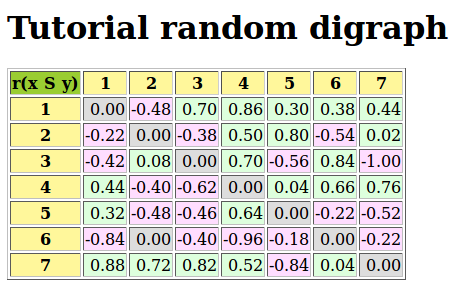
\includegraphics[width=7cm]{Figures/2-6-htmlTutorialDigraph.png}
\caption{The valued relation table shown in a browser window. Positive arcs are shown in green and negative arcs in red. Indeterminate --zero-valued-- links, like the reflexive diagonal ones or the link between node \texttt{'6'} and node \texttt{'2'}, are shown in gray}
\label{fig:2.6}       % Give a unique label
\end{figure}
 
\section{Complete, empty and indeterminate digraphs}
\label{sec:2.10}

Let us finally mention some special universal classes of digraphs that are readily available in the \texttt{digraphs} module\footnote{See \citealp{BIS-2021}}, like:
\begin{itemize}[nosep]
\item the \texttt{CompleteDigraph}\index{CompleteDigraph@\texttt{CompleteDigraph} class},
\item  the \texttt{EmptyDigraph}\index{EmptyDigraph@\texttt{EmptyDigraph} class} and
\item  the \texttt{IndeterminateDigraph}\index{IndeterminateDigraph@\texttt{IndeterminateDigraph} class} class,
\end{itemize}
who put all characteristic values respectively to the \emph{maximum}, the \emph{minimum} or the \emph{median} indeterminate characteristic value.
\begin{lstlisting}[caption={Complete, empty and indeterminate digraphs},label=list:2.11]
>>> from digraphs import CompleteDigraph,EmptyDigraph,\
...   			 IndeterminateDigraph
>>> # the empty digraph   
>>> e = EmptyDigraph(order=5)
>>> e.showRelationTable()
    * ---- Relation Table -----
      S   |    '1'    '2'    '3'    '4'	   '5'	  
    ---- -|-----------------------------------
    '1'   |  -1.00  -1.00  -1.00  -1.00	 -1.00	 
    '2'   |  -1.00  -1.00  -1.00  -1.00	 -1.00	 
    '3'   |  -1.00  -1.00  -1.00  -1.00	 -1.00	 
    '4'   |  -1.00  -1.00  -1.00  -1.00	 -1.00	 
    '5'   |  -1.00  -1.00  -1.00  -1.00	 -1.00
>>> e.showNeighborhoods() 
    Neighborhoods:
      Gamma     :
    '1': in => set(), out => set()
    '2': in => set(), out => set()
    '5': in => set(), out => set()
    '3': in => set(), out => set()
    '4': in => set(), out => set()
      Not Gamma :
    '1': in => {'2','4','5','3'}, out => {'2','4','5','3'}
    '2': in => {'1','4','5','3'}, out => {'1','4','5','3'}
    '5': in => {'1','2','4','3'}, out => {'1','2','4','3'}
    '3': in => {'1','2','4','5'}, out => {'1','2','4','5'}
    '4': in => {'1','2','5','3'}, out => {'1','2','5','3'}
>>> # the indeterminate digraph
>>> i = IndeterminateDigraph()
    * ---- Relation Table -----
      S   |   '1'   '2'	  '3'	'4'   '5'	  
    ------|------------------------------
    '1'   |  0.00  0.00	 0.00  0.00  0.00	 
    '2'   |  0.00  0.00	 0.00  0.00  0.00	 
    '3'   |  0.00  0.00	 0.00  0.00  0.00	 
    '4'   |  0.00  0.00	 0.00  0.00  0.00	 
    '5'   |  0.00  0.00	 0.00  0.00  0.00	 
>>> i.showNeighborhoods()
    Neighborhoods:
      Gamma     :
    '1': in => set(), out => set()
    '2': in => set(), out => set()
    '5': in => set(), out => set()
    '3': in => set(), out => set()
    '4': in => set(), out => set()
      Not Gamma :
    '1': in => set(), out => set()
    '2': in => set(), out => set()
    '5': in => set(), out => set()
    '3': in => set(), out => set()
    '4': in => set(), out => set()
\end{lstlisting}

Mind the subtle difference between the neighbourhoods of an \emph{empty} and the neighbourhoods of an \emph{indeterminate} digraph instance. In the first kind, the neighbourhoods are known to be completely \emph{empty}  (see List.~\vref{list:2.11} Lines 22-27) whereas, in the latter, \emph{nothing is known} about the actual neighbourhoods of the nodes  (see Lines 46-51). These two cases illustrate why in the case of \emph{bipolar-valued} digraphs, we may sometimes need both a \texttt{gamma} \textbf{and} a \texttt{notGamma} attribute.

\vspace{1cm}
In the following Chapter~\ref{sec:3}  we introduce the main formal object of this book, namely \emph{bipolar-valued outranking} digraphs.

%%%%%%%%%%%%%%%%%%%%%%%%%%%%%%%%%%%%
\phantomsection
\addcontentsline{toc}{section}{Notes}
\section*{Notes}

It is \emph{D. Bouyssou} \index{Bouyssou@\emph{D. Bouyssou}} who first suggested us end of the nineties, when we started to work in Prolog on the computation of digraph kernels with finite domain constraint solvers, that the $50\%$ criteria significance majority was a special value to be carefully taken into account. The converging solution vectors of the fixpoint kernel equations confirmed this special status of the $50\%$ majority (see Chap.~\ref{sec:17}). These early insights led to the seminal articles on bipolar-valued epistemic logic where we introduced split truth/falseness semantics for a multi-valued logical processing of fuzzy preference modelling \citep{BIS-2000,BIS-2002}. The characteristic valuation domain remained however the classical fuzzy $[0.0;1.0]$ valuation domain.

It is only in 2004, when we succeeded in assessing the stability of the outranking digraph when solely ordinal criteria significance weights are given, that it became clear and evident for us that the characteristic valuation domain had to be shifted to a bipolar $[-1.0;+1.0]$-valued domain \citep{BIS-2004a}. In this bipolar valuation domain, the $50\%$ majority thershold corresponds now to the median $0.0$ value, characterising with the correct zero value an epistemic indetermination --no knowledge-- situation. Furthermore, identifying truth and falseness by the sign of the characteristic values revealed itself to be very efficient not only from a computational point of view, but also from scientific and semiotical perspectives. A positive (resp. negative) characteristic value now attest a logically valid (resp. invalid) statement and a negative affirmation now corresponds to a positive refutation. Furthermore, the median zero value gives way to efficiently handling partial digraphs --like the border or the assymetric part of a digraph-- and, even more important from a practical decision making point of view, any missing data.

The bipolar $[-1.0;+1.0]$-valued characteritisc domain opened so the way to important new operations and concepts, like the disjunctive epistemic fusion operation seen in Section~\vref{sec:2.5} that confers the outranking digraph a logically and epistemically sound definition \citep{BIS-2013}. \Kendall 's ordinal correlation index could be extended to a bipolar-valued relational equivalence index between digraphs \citep{BIS-2012a}. Making usage of the bipolar-valued Gaussian error function naturally led to defining a bipolar-valued likelihood function, where a positive (resp. negative) value gives the likelihood of an affirmation (resp. a refutation) \citep{BIS-2014}.      

%%%%%%% The chapter bibliography
%\normallatexbib
%\clearpage
%\phantomsection
%\addcontentsline{toc}{section}{Chapter Bibliograhy}
\bibliographystyle{spbasic}
%\typeout{}
\bibliography{03-backMatters/reference}
%\chapter{Working with bipolar-valued digraphs}
\label{sec:2}

\abstract*{ The chapter introduces bipolar-valued digraphs, the fondamental root type of all the specialised digraphs implemented in the \Digraph modules. With the help of a randomly valued digraph, we illustrate some basic digraph manipulation methods, like drawing the digraph, dividing the digraph into its asymmetric and symmetric parts, separating the border from the inner part, computing associated dual, converse and codual digraphs, and operating symmetric and transitive closures.}

\abstract{ The chapter introduces bipolar-valued digraphs, the fondamental root type of all the specialised digraphs implemented in the \Digraph modules. With the help of a randomly valued digraph, we illustrate some basic digraph manipulation methods, like drawing the digraph, dividing the digraph into its asymmetric and symmetric parts, separating the border from the inner part, computing associated dual, converse and codual digraphs, and operating symmetric and transitive closures.}

\section{Random bipolar-valued digraphs}

In Listing~\vref{list:2.1}, we generate a uniformly random $[-1.0; +1.0]$-valued digraph of order 7, denoted \texttt{rdg} and modelling, for instance, a binary relation $S(x,y)$ defined on the set of nodes of \texttt{rdg}. For this purpose, the \Digraph resources provide in the \texttt{randomDigraphs}\index{randomDigraphs@\texttt{randomDigraphs} module} module a specific \texttt{RandomValuationDigraph}\index{RandomValuationDigraph@\texttt{RandomValuationDigraph} class} class \citep{BIS-2021b}.
\begin{lstlisting}[caption={Random bipolar-valued digraph instance},label=list:2.1]
>>> from randomDigraphs import RandomValuationDigraph
>>> rdg = RandomValuationDigraph(order=7)
>>> rdg.save('tutRandValDigraph')
>>> from digraphs import Digraph
>>> rdg = Digraph('tutRandValDigraph')
>>> rdg
  *------- Digraph instance description ------*
   Instance class      : Digraph
   Instance name       : tutRandValDigraph
   Digraph Order       : 7
   Digraph Size        : 22
   Valuation domain    : [-1.00;1.00]
   Determinateness (%) : 75.24
   Attributes          : ['name','actions','order',
                          'valuationdomain','relation',
                          'gamma','notGamma']
\end{lstlisting}   

With the \texttt{save()} \index{save@\texttt{save()}} method (see Line 3) we keep for future use a backup version of \texttt{rdg} which is saved into a file named \texttt{tutRandValDigraph.py} in the current working directory. The genuine \texttt{Digraph} class constructor may restore the \texttt{rdg} object from the stored file (Lines 4-5). We may easily inspect the content of \texttt{rdg} (Line 6). The digraph size 22 indicates the number of positively valued arcs. The valuation domain is uniformly distributed in the interval $[-1.0; 1.0]$ and the mean absolute arc valuation is $(0.7524 \times 2)\, -\, 1.0 \;=\; 0.5048$ (Line 13).

As mentioned in the previous Chapter~\ref{sec:1}, all objects of \texttt{Digraph} type contain at least the list of attributes shown here in Lines 14-16: --a \texttt{name} (string), --a dictionary of \texttt{actions} (digraph nodes), --an \texttt{order} (integer) attribute containing the number of actions, --a \texttt{valuationdomain} dictionary, --a double dictionary \texttt{relation} representing the adjacency table of the digraph relation, --a \texttt{gamma} and --a {\tt notGamma} dictionary containing the direct neighbourhood of each action.

The \texttt{Digraph} class provides some generic \texttt{show...()} methods for exploring the content of a given \texttt{ Digraph} object, like the \texttt{showRelationTable()}\index{showRelationTable@\texttt{showRelationTable()}}, the \texttt{showComponents()}\index{showComponents@\texttt{showComponents()}} and the \texttt{showNeighborhoods()}\index{showNeighborhoods@\texttt{showNeighborhoods()}} methods.
\begin{lstlisting}[caption={Example of random valuation digraph},label=list:2.2]
>>> rdg.showRelationTable()
  * ---- Relation Table -----
   r(xSy) |  '1'    '2'   '3'  '4'   '5'    '6'  '7'	  
   -------|-------------------------------------------
    '1'   |  0.00 -0.48  0.70  0.86  0.30  0.38  0.44	 
    '2'   | -0.22  0.00 -0.38  0.50  0.80 -0.54  0.02	 
    '3'   | -0.42  0.08  0.00  0.70 -0.56  0.84 -1.00	 
    '4'   |  0.44 -0.40 -0.62  0.00  0.04  0.66  0.76	 
    '5'   |  0.32 -0.48 -0.46  0.64  0.00 -0.22 -0.52	 
    '6'   | -0.84  0.00 -0.40 -0.96 -0.18  0.00 -0.22	 
    '7'   |  0.88  0.72  0.82  0.52 -0.84  0.04  0.00
>>> rdg.showComponents()
  *--- Connected Components ---*
  1: ['1', '2', '3', '4', '5', '6', '7']
>>> rdg.showNeighborhoods()
  *---- Neighborhoods ------*
     Gamma:
     '1': in => {'5','7','4'}, out => {'5','7','6','3','4'}
     '2': in => {'7','3'},out => {'5','7','4'}
     '3': in => {'7','1'}, out => {'6','2','4'}
     '4': in => {'5','7','1','2','3'}, out => {'5','7','1','6'}
     '5': in => {'1','2','4'}, out => {'1','4'}
     '6': in => {'7','1','3','4'}, out => set()
     '7': in => {'1','2','4'}, out => {'1','2','3','4','6'}
     Not Gamma:
     '1': in => {'6','2','3'}, out => {'2'}
     '2': in => {'5','1','4'}, out => {'1','6','3'}
     '3': in => {'5','6','2','4'}, out => {'5','7','1'}
     '4': in => {'6'}, out => {'2','3'}
     '5': in => {'7','6','3'}, out => {'7','6','2','3'}
     '6': in => {'5','2'}, out => {'5','7','1','3','4'}
     '7': in => {'5','6','3'}, out => {'5'}
\end{lstlisting}   

Mind that some \texttt{Digraph} class methods will ignore the \emph{reflexive} links by considering that they are \emph{indeterminate}, i.e. the characteristic value $r(x\,S\,x)$ for all action $x$ is set to the \emph{median}, i.e. \emph{indeterminate} value $0.0$ in this case (see Listing~\vref{list:2.2} Lines 5-11 and \citet{BIS-2004a}).

\section{Graphviz drawings}
\label{sec:2.2}

An even better insight into the \texttt{Digraph} object \texttt{rdg} is given by looking at its \href{https://graphviz.org/}{graphviz} drawing \citep{graphviz}\footnote{The \texttt{exportGraphViz()} method is depending on drawing tools from the graphviz software (https://graphviz.org/). On Linux Ubuntu or Debian you may try \texttt{sudo apt-get install graphviz} to install them. There are ready \emph{dmg} installers for Mac OSX.}\index{graphviz}.
\begin{lstlisting}
>>> rdg.exportGraphViz('tutRandValDigraph')
 *---- exporting a dot file for GraphViz tools ------*
  Exporting to tutRandValDigraph.dot
  dot -Grankdir=BT -Tpng tutRandValDigraph.dot\
                           -o tutRandValDigraph.png
\end{lstlisting}
\begin{figure}[ht]
\sidecaption[t]
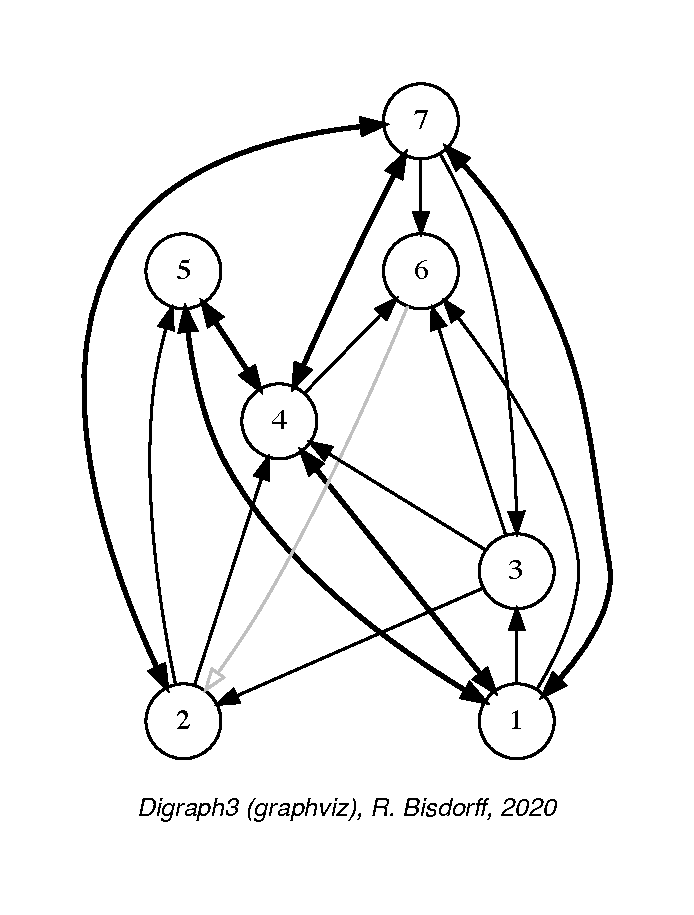
\includegraphics[width=6cm]{Figures/2-1-tutRandValDigraph.pdf}
\caption{\emph{The tutorial random valuation digraph}. Double links are drawn in bold black with an arrowhead at each end, whereas single asymmetric links are drawn in black with an arrowhead showing the direction of the link. Notice the undetermined relational situation ($r(6\,S\,2) = 0.00$) observed between nodes '6' and '2'. The corresponding link is marked in gray with an open arrowhead in the drawing}
\label{fig:2.1}       % Give a unique label
\end{figure}
  
\section{Asymmetric and symmetric parts}
\label{sec:2.3}

We may now extract both the \emph{}\emph{symmetric} as well as the \emph{asymmetric} part of digraph \texttt{rdg} with the help of two corresponding constructors (see List.~\vref{list:2.3}) \index{AsymmetricPartialDigraph@\texttt{AsymmetricPartialDigraph} class}\index{SymmetricPartialDigraph@\texttt{SymmetricPartialDigraph} class}.
\begin{lstlisting}[caption={Computing asymmetric and symmetric Parts},label=list:2.3]
>>> from digraphs import AsymmetricPartialDigraph,\
...                      SymmetricPartialDigraph
>>> asymDg = AsymmetricPartialDigraph(rdg)
>>> asymDg.exportGraphViz()
>>> symDg = SymmetricPartialDigraph(rdg)
>>> symDg.exportGraphViz()
\end{lstlisting}
\begin{figure}[ht]
  % \sidecaption
  Asymmetric Part \hfill Symmetric Part \\
  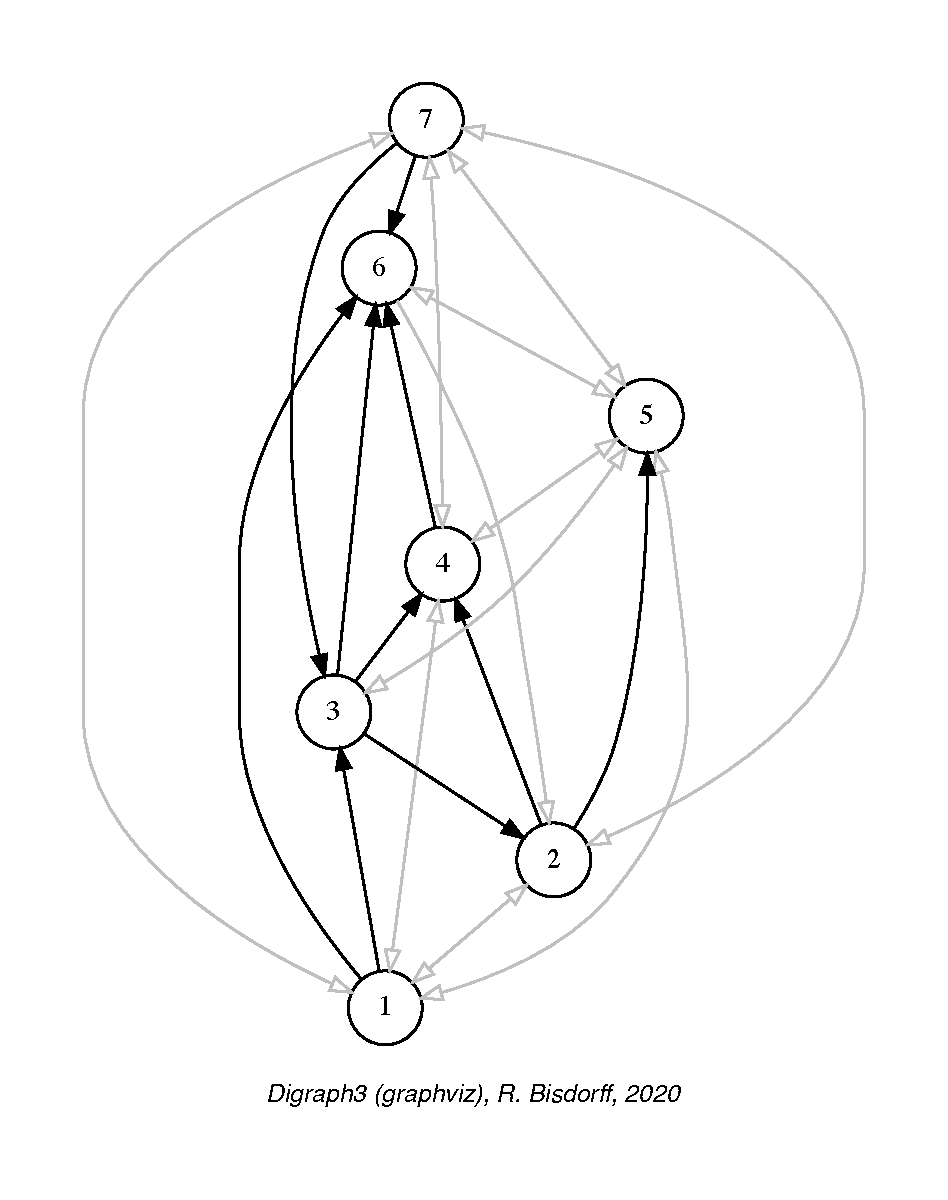
\includegraphics[height=6cm]{Figures/2-2-asymmetricPart.pdf}\hfill
  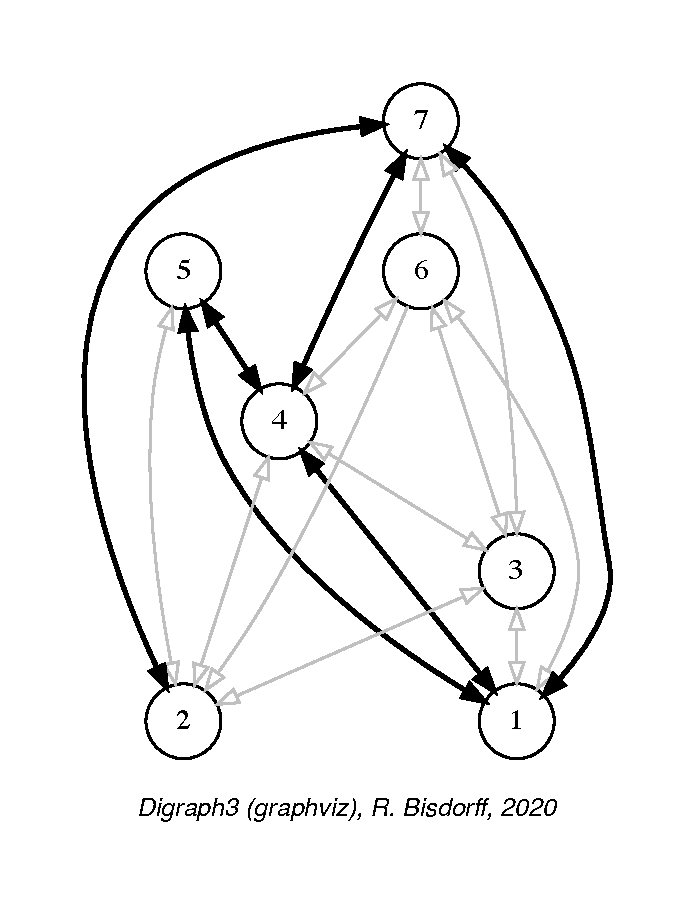
\includegraphics[height=6cm]{Figures/2-2-symmetricPart.pdf}\hfill
\caption{Asymmetric and symmetric part of the tutorial random valuation digraph}
\label{fig:2.2}       % Give a unique label
\end{figure}

The constructor of the partial objects \texttt{asymDg} and \texttt{symDg} puts to the indeterminate characteristic value all non-asymmetric, respectively non-symmetric links between nodes (see Fig.~\vref{fig:2.2}).

Here below, for illustration the source code of the \texttt{ relation} constructor of the \texttt{AsymmetricPartialDigraph} class.
\begin{lstlisting}[caption={Computing the asymmetric part of a bipolar-valued relation},label=list:2.4,basicstyle=\ttfamily\scriptsize]
def _constructRelation(self):
    actions = self.actions
    Min = self.valuationdomain['min']
    Max = self.valuationdomain['max']
    Med = self.valuationdomain['med']
    relationIn = self.relation
    relationOut = {}
    for a in actions:
	relationOut[a] = {}
	for b in actions:
	    if a != b:
                if relationIn[a][b] >= Med and relationIn[b][a] <= Med:
		    relationOut[a][b] = relationIn[a][b]
		elif relationIn[a][b] <= Med and relationIn[b][a] >= Med:
		    relationOut[a][b] = relationIn[a][b]
		else:
		    relationOut[a][b] = Med
	    else: # reflexive links are ignored
		relationOut[a][b] = Med
    return relationOut
\end{lstlisting}

\section{Border and inner parts}
\label{sec:2.4}

We may also extract the \emph{border} --the part of a digraph induced by the union of its initial and terminal prekernels (see Chap.~\ref{sec:17})--  as well as, the \emph{inner part} --the complement of the border-- with the help of two corresponding class constructors: \texttt{GraphBorder}\index{GraphBorder@\texttt{GraphBorder} class} and \texttt{GraphInner}\index{GraphInner@\texttt{GraphInner} class} (see Fig.~\vref{fig:2.3}).

\begin{figure}[ht]
%\sidecaption
  Border Part \hfill Inner Part \\
  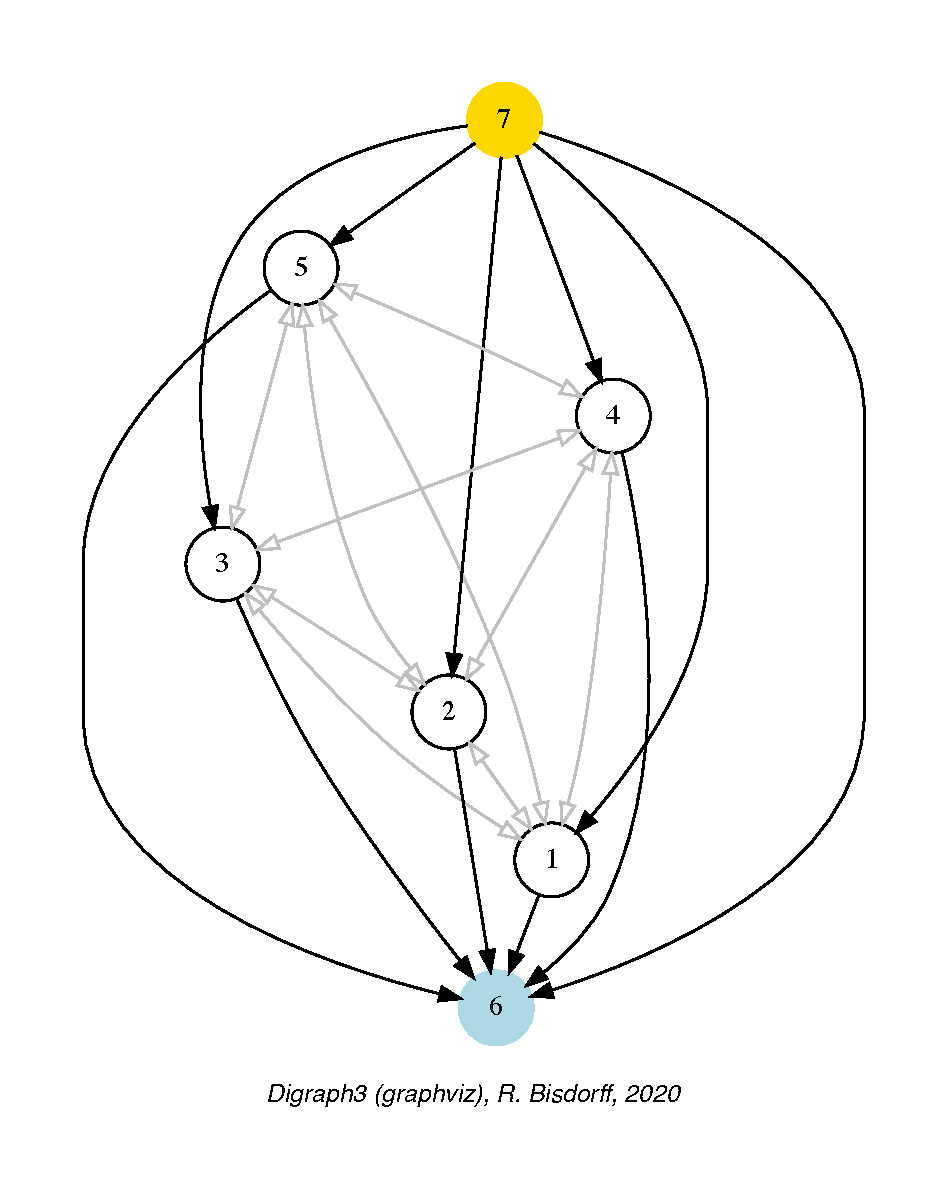
\includegraphics[height=6cm]{Figures/2-3-linearOrderBorder.pdf}\hfill
  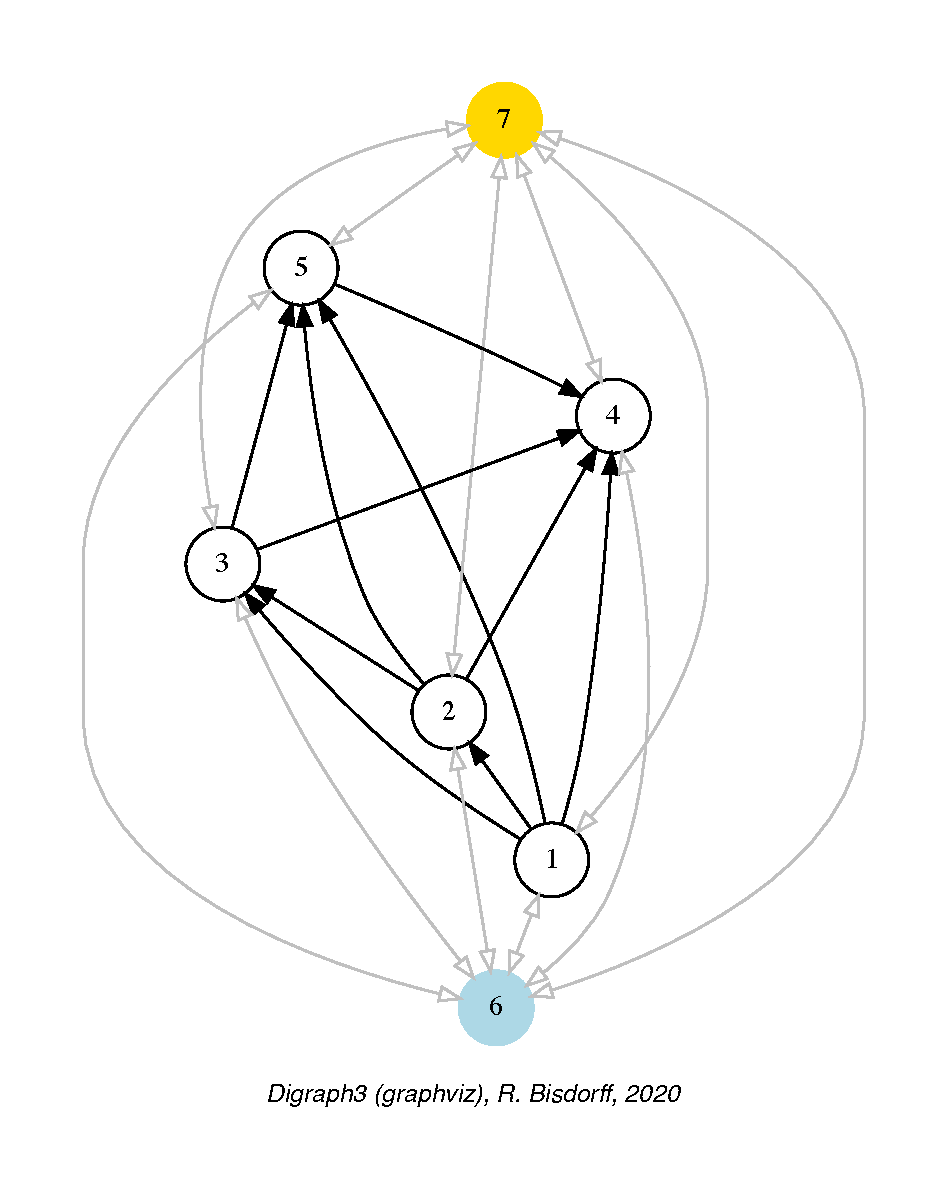
\includegraphics[height=6cm]{Figures/2-3-linearOrderInner.pdf}\hfill
\caption{\emph{Border} and \emph{inner} part of a linear order oriented by \emph{terminal} and \emph{initial} kernels.}
\label{fig:2.3}       % Give a unique label
\end{figure}
Let us illustrate the digraph border and inner parts on a linear ordering obtained from the tutorial random valuation digraph \texttt{rdg}  with the \NetFlows ranking rule  (see Sec.~\ref{sec:8.3}).  
\begin{lstlisting}[caption={Border and inner part of a linear order},label=list:2.5]
>>> from digraphs import GraphBorder, GraphInner
>>> from linearOrders import NetFlowsOrder
>>> nf = NetFlowsOrder(rdg)
>>> nf.netFlowsOrder
   ['6', '4', '5', '3', '2', '1', '7']
>>> bnf = GraphBorder(nf)
>>> bnf.exportGraphViz(lastChoice=['6'],firstChoice=['7'])
>>> inf = GraphInner(nf)
>>> inf.exportGraphViz(lastChoice=['6'],firstChoice=['7'])
\end{lstlisting}
We may orient the \texttt{graphviz} drawings in Figure~\vref{fig:2.3}  with the terminal node 6 (\texttt{lastChoice} parameter) and initial node 7 (\texttt{firstChoice} parameter) (see List.~\vref{list:2.5} Lines 7 and 9).

The constructor of the partial digraphs \texttt{bnf} and \texttt{inf}  (see Lines 3 and 6) puts to the \emph{indeterminate} characteristic value all links not in the \emph{border}, respectively \emph{not} in the \emph{inner} part (see Fig.~\vref{fig:2.3}). Being much {\em denser\/} than a linear order, the actual inner part of our tutorial random valuation digraph \texttt{rdg} is reduced to a single arc between nodes 3 and 4 (see Fig.~\vref{fig:2.4}). Indeed, a complete digraph on the limit has no inner part (privacy!) at all, whereas empty and indeterminate digraphs admit both, an empty border and an empty inner part.
\begin{figure}[h]
%\sidecaption
  Border Part \hfill Inner Part \\
  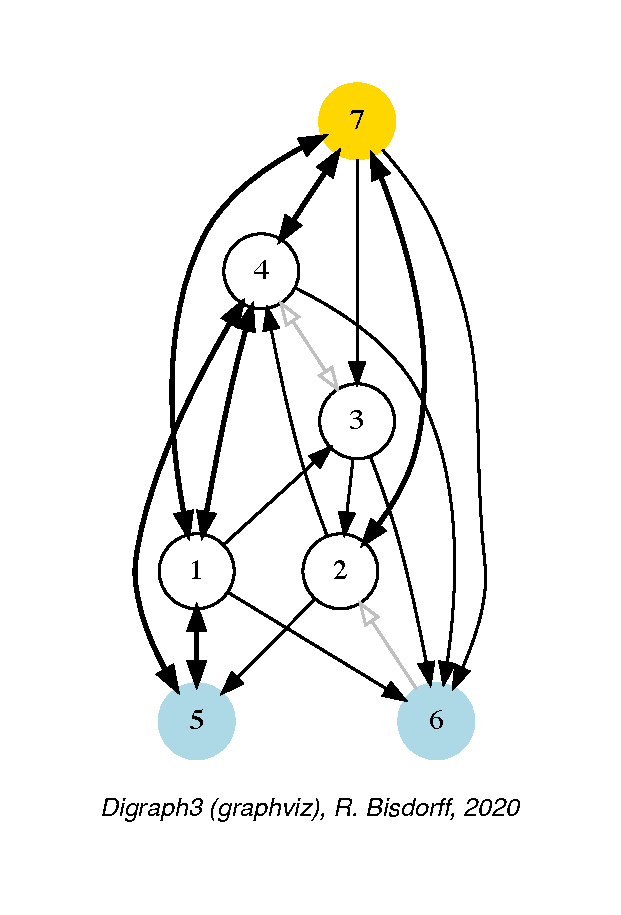
\includegraphics[height=6cm]{Figures/2-4-tutRandValDigraph_border.pdf}\hfill
  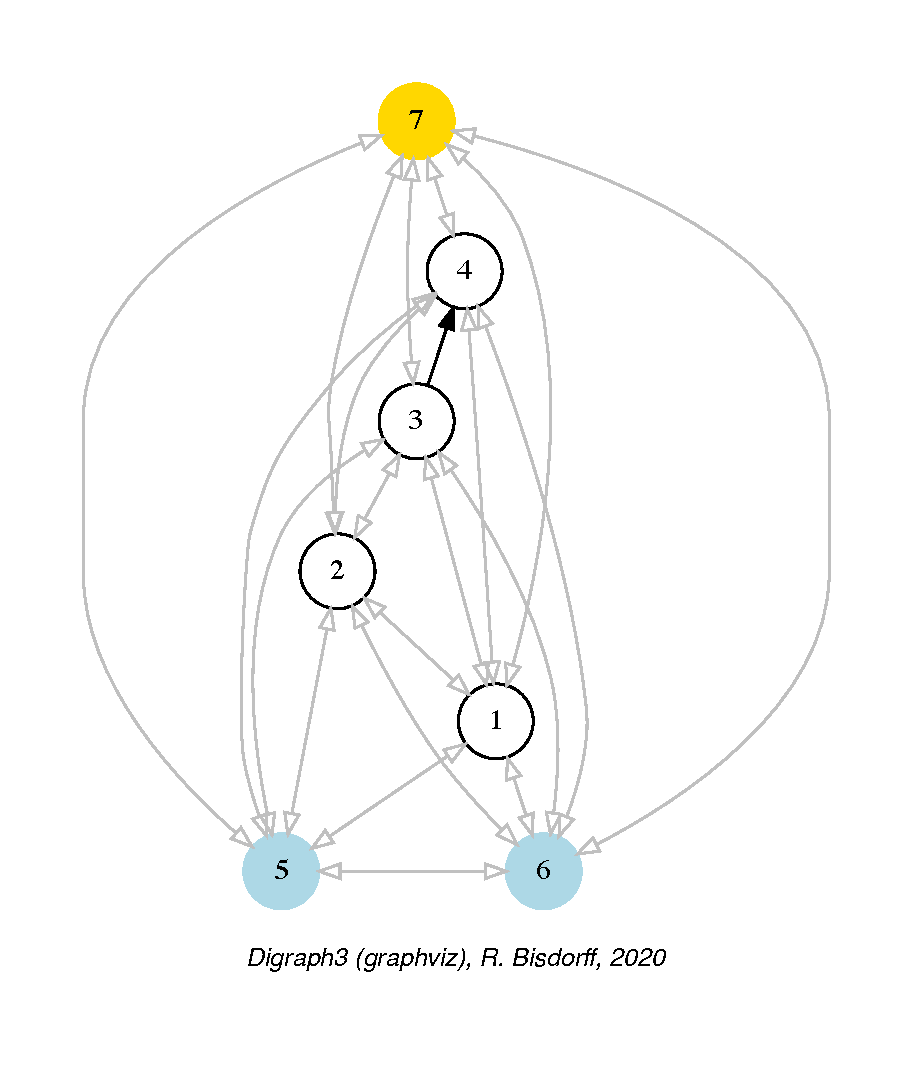
\includegraphics[height=6cm]{Figures/2-4-tutRandValDigraph_inner.pdf}\hfill
\caption{Border and inner part of the tutorial random valuation digraph \texttt{rdg}}
\label{fig:2.4}       % Give a unique label
\end{figure}

\section{Fusion by epistemic disjunction}
\label{sec:2.5}

We may recover object \texttt{rdg} from both partial objects \texttt{asymDg} and \texttt{symDg}, or as well from the border \texttt{bg} and the inner part \texttt{ig}, with a \emph{bipolar fusion} operator, also called \emph{epistemic disjunction}, available via the \texttt{FusionDigraph}\index{FusionDigraph@\texttt{FusionDigraph} class} class. 
\begin{lstlisting}[caption={Epistemic fusion of partial diagraphs},label=list:2.6]
>>> from digraphs import FusionDigraph
>>> fusDg = FusionDigraph(asymDg,symDg,operator='o-max')
>>> # fusDg = FusionDigraph(bg,ig,operator='o-max')
>>> fusDg.showRelationTable()
  * ---- Relation Table -----
   r(xSy) |  '1'    '2'   '3'  '4'   '5'    '6'  '7'	  
   -------|------------------------------------------
    '1'   |  0.00 -0.48  0.70  0.86  0.30  0.38  0.44	 
    '2'   | -0.22  0.00 -0.38  0.50  0.80 -0.54  0.02	 
    '3'   | -0.42  0.08  0.00  0.70 -0.56  0.84 -1.00	 
    '4'   |  0.44 -0.40 -0.62  0.00  0.04  0.66  0.76	 
    '5'   |  0.32 -0.48 -0.46  0.64  0.00 -0.22 -0.52	 
    '6'   | -0.84  0.00 -0.40 -0.96 -0.18  0.00 -0.22	 
    '7'   |  0.88  0.72  0.82  0.52 -0.84  0.04  0.00
\end{lstlisting}

The epistemic fusion operator \texttt{o-max} (see List.~\vref{list:2.6} Line 2) is defined as follows:
\begin{definition}[Disjunctive epistemic fusion operator \texttt{o-max}]\label{def:disjunctiveFusion}

\noindent Let $r$ and $r'$ characterise two bipolar-valued epistemic situations:
\begin{itemize}[leftmargin=0.5cm,rightmargin=0.5cm,nosep]
\item \texttt{o-max}$(r, r')$ = $\max(r, r' )$ when both $r$ and $r'$ are more or less valid or indeterminate;
\item \texttt{o-max}$(r, r')$ = $\min(r, r' )$ when both $r$ and $r'$ are more or less invalid or indeterminate;
\item \texttt{o-max}$(r, r')$ = $0.0$, i.e. indeterminate otherwise.
\end{itemize}
\end{definition}

Mind that the \texttt{o-max} operator, like a mean operator, is \emph{not associative} when more than 2 operands are given. In order to make the \texttt{o-max} fusion univocal, the following rule is applied: --first, all positive and negative terms are separately aggregated, --then the \texttt{o-max} fusion is applied on both aggregates.

\section{Dual, converse and codual digraphs}
\label{sec:2.6}

We may as readily compute the \emph{dual}\index{DualDigraph@\texttt{DualDigraph} class} (negated relation \footnote{Not to be confused with the dual graph of a plane graph $g$ that has a vertex for each face of $g$. Here we mean the \emph{less than} (strict converse) relation corresponding to a \emph{greater or equal} relation, or the \emph{less than or equal} relation corresponding to a (strict) \emph{better than} relation.}), the \emph{converse}\index{ConverseDigraph@\texttt{ConverseDigraph} class} (transposed relation) and the \emph{codual}\index{CoDualDigraph@\texttt{CoDualDigraph} class} (transposed and negated relation) of the digraph instance \texttt{rdg}. 
\begin{lstlisting}[caption={Computing associated dual, converse and codual digraphs},label=list:2.7]
>>> from digraphs import\
...          DualDigraph, ConverseDigraph, CoDualDigraph
>>> # dual of rdg
>>> ddg = DualDigraph(rdg)
>>> ddg.showRelationTable()
    -r(xSy) |  '1'    '2'   '3'  '4'   '5'    '6'  '7'	  
    --------|------------------------------------------
    '1 '    |  0.00  0.48 -0.70 -0.86 -0.30 -0.38 -0.44	 
    '2'     |  0.22  0.00  0.38 -0.50  0.80  0.54 -0.02	 
    '3'     |  0.42  0.08  0.00 -0.70  0.56 -0.84  1.00	 
    '4'     | -0.44  0.40  0.62  0.00 -0.04 -0.66 -0.76	 
    '5'     | -0.32  0.48  0.46 -0.64  0.00  0.22  0.52	 
    '6'     |  0.84  0.00  0.40  0.96  0.18  0.00  0.22	 
    '7'     |  0.88 -0.72 -0.82 -0.52  0.84 -0.04  0.00
>>> # converse of rdg
>>> cdg = ConverseDigraph(rdg)
>>> cdg.showRelationTable()
    * ---- Relation Table -----
     r(ySx) |  '1'    '2'   '3'   '4'   '5'   '6'   '7'	  
    --------|------------------------------------------
    '1'     |  0.00 -0.22 -0.42  0.44  0.32 -0.84  0.88	 
    '2'     | -0.48  0.00  0.08 -0.40 -0.48  0.00  0.72	 
    '3'     |  0.70 -0.38  0.00 -0.62 -0.46 -0.40  0.82	 
    '4'     |  0.86  0.50  0.70  0.00  0.64 -0.96  0.52	 
    '5'     |  0.30  0.80 -0.56  0.04  0.00 -0.18 -0.84	 
    '6'     |  0.38 -0.54  0.84  0.66 -0.22  0.00  0.04	 
    '7'     |  0.44  0.02 -1.00  0.76 -0.52 -0.22  0.00	 
>>> # codual of rdg
>>> cddg = CoDualDigraph(rdg)
>>> cddg.showRelationTable()
    * ---- Relation Table -----
    -r(ySx) |  '1'    '2'   '3'   '4'   '5'   '6'   '7'	    
    --------|------------------------------------------
    '1'     |  0.00  0.22  0.42 -0.44 -0.32  0.84 -0.88	 
    '2'     |  0.48  0.00 -0.08  0.40  0.48  0.00 -0.72	 
    '3'     | -0.70  0.38  0.00  0.62  0.46  0.40 -0.82	 
    '4'     | -0.86 -0.50 -0.70  0.00 -0.64  0.96 -0.52	 
    '5'     | -0.30 -0.80  0.56 -0.04  0.00  0.18  0.84	 
    '6'     | -0.38  0.54 -0.84 -0.66  0.22  0.00 -0.04	 
    '7'     | -0.44 -0.02  1.00 -0.76  0.52  0.22  0.00	 
\end{lstlisting}

Computing the \emph{dual}, respectively the \emph{converse} of a digraph, may also be done with prefixing the \texttt{\_\_neg\_\_} ($-$) or the \texttt{\_\_invert\_\_} ($\sim$) operator. The \emph{codual} of a \texttt{Digraph} object may, hence, as well be computed with a \emph{composition} (in either order) of both operations.
\begin{lstlisting}[caption={Computing the dual, the converse and the codual of a digraph},label=list:2.8]
>>> ddg = -rdg   # dual of rdg
>>> cdg = ~rdg   # converse of rdg
>>> cddg = ~(-rdg) # = -(~(rdg) codual of rdg
>>> (-(~rdg)).showRelationTable()
  * ---- Relation Table -----
   -r(ySx) |  '1'    '2'   '3'   '4'   '5'   '6'   '7'	    
   --------|------------------------------------------
   '1'     |  0.00  0.22  0.42 -0.44 -0.32  0.84 -0.88	 
   '2'     |  0.48  0.00 -0.08  0.40  0.48  0.00 -0.72	 
   '3'     | -0.70  0.38  0.00  0.62  0.46  0.40 -0.82	 
   '4'     | -0.86 -0.50 -0.70  0.00 -0.64  0.96 -0.52	 
   '5'     | -0.30 -0.80  0.56 -0.04  0.00  0.18  0.84	 
   '6'     | -0.38  0.54 -0.84 -0.66  0.22  0.00 -0.04	 
   '7'     | -0.44 -0.02  1.00 -0.76  0.52  0.22  0.00	 
\end{lstlisting}
  
\section{Symmetric and transitive closures}
\label{sec:2.7}

Symmetric and transitive closures, by default in-site methods, are also available (see Fig.~\vref{fig:2.5})\index{closeSymmetric@\texttt{closeSymmetric()}}\index{closeTransitive@\texttt{closeTransitive()}}. Note that it is a good idea, before going ahead with these in-site operations, who irreversibly modify the original \texttt{rdg} object, to previously make a backup version of \texttt{rdg}. The simplest storage method, always provided by the generic \texttt{Digraph.save()} method, writes out in a named file the python content of the Digraph object in string representation (see Sec.~\vref{sec:1.3}).
\begin{lstlisting}[caption={Symmeric and transitive closures},label=list:2.9]
>>> rdg.save('tutRandValDigraph')
>>> rdg.closeSymmetric(InSite=True)
>>> rdg.closeTransitive(InSite=True)
>>> rdg.exportGraphViz('strongComponents')
\end{lstlisting}
\begin{figure}[h]
\sidecaption[t]
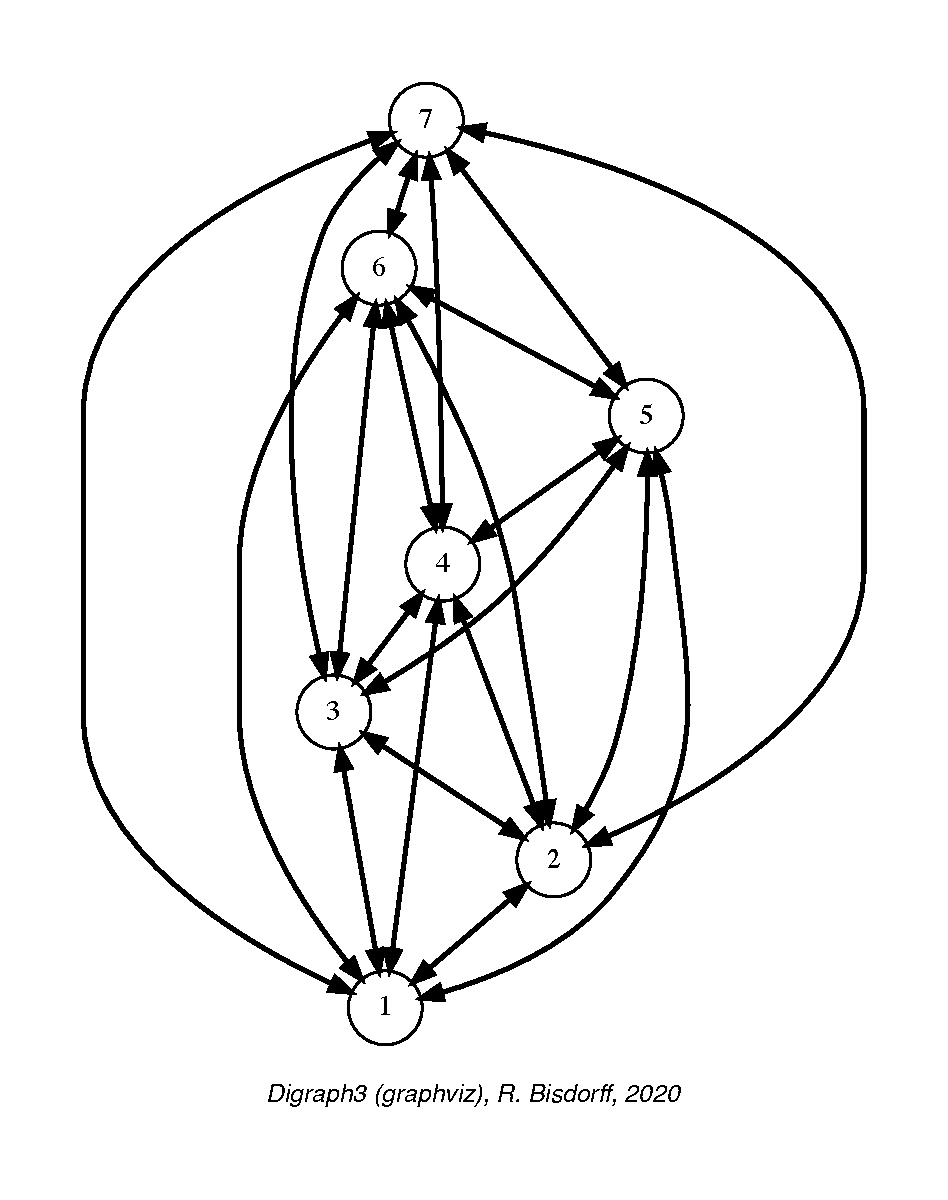
\includegraphics[width=6cm]{Figures/2-5-strongComponents.pdf}
\caption{Symmetric and transitive closure of the tutorial random valuation digraph $rdg$.}
\label{fig:2.5}       % Give a unique label
\end{figure}

The \texttt{closeSymmetric()}\index{closeSymmetric@\texttt{closeSymmetric()}} method (see List.~\vref{list:2.9} Line 2), of complexity $O(n^2)$ where $n$ denotes the digraph's order, changes, on the one hand, all single pairwise links it may detect into double links by operating a disjunction of the pairwise relations. On the other hand, the \texttt{closeTransitive()}\index{closeTransitive@\texttt{closeTransitive()}}  method (see Line 3), implements the \emph{Roy-Warshall} transitive closure algorithm of complexity $O(n^3)$ \index{Roy@\textsl{B. Roy}} \index{warshall@\textsl{S. Warshall}} (\citealp{ROY-1959} and \citealp{WAR-1962}).

The same \texttt{closeTransitive()} with a \texttt{Reverse = True} flag may be readily used for eliminating all transitive arcs from a transitive digraph instance. We make usage of this feature when drawing Hasse diagrams of \texttt{TransitiveDigraph}\index{TransitiveDigraph@\texttt{TransitiveDigraph} class} objects.

\section{Strong components}
\label{sec:2.8}

As the original digraph \texttt{rdg} was connected (see above the result of the showShort() command), both the symmetric and the transitive closures operated together, will necessarily produce a single strong component, i.e. a \textbf{complete} digraph. We may sometimes wish to collapse all strong components in a given digraph and construct the so \emph{collapsed} digraph. Using the \texttt{StrongComponentsCollapsedDigraph} constructor \index{StrongComponentsCollapsedDigraph@\texttt{StrongComponentsCollapsedDigraph} class} here will render a single hyper-node gathering all the original nodes (see Line 7 below).
\begin{lstlisting}[caption={Computing the strong components in a digraph},label=list:2.10]
>>> from digraphs import StrongComponentsCollapsedDigraph
>>> sc = StrongComponentsCollapsedDigraph(rdg)
>>> sc.showAll()
  *----- show detail -----*
   Digraph          : tutRandValDigraph_Scc
  *---- Actions ----*
    ['_7_1_2_6_5_3_4_']
  *---- Relation Table -----
      S     |  'Scc_1'	  
     -------|---------
     'Scc_1' |  0.00
  *---- strong Components ----*
   short 	 content
   'Scc_1' 	 '_7_1_2_6_5_3_4_'
  *---- Neighborhoods ----*
   Gamma     :
   'frozenset({'7','1','2','6','5','3','4'})':
                     in => set(), out => set()
   Not Gamma :
   'frozenset({'7','1','2','6','5','3','4'})':
                     in => set(), out => set()
\end{lstlisting}
  
\section{CSV storage}
\label{sec:2.9}

Sometimes it is required to exchange the graph valuation data in CSV format with a statistical package like \textbf{R}\footnote{\url{https://www.r-project.org/}}. For this purpose it is possible to export the digraph data into a CSV file. The valuation domain is hereby normalised by default to the range $[-1.0,1.0]$ and the diagonal is put by default to the minimal value $-1.0$.
\begin{lstlisting}
>>> rdg = Digraph('tutRandValDigraph')
>>> rdg.saveCSV('tutRandValDigraph')
  # content of file tutRandValDigraph.csv
  "d","1","2","3","4","5","6","7"
  "1",-1.0,0.48,-0.7,-0.86,-0.3,-0.38,-0.44
  "2",0.22,-1.0,0.38,-0.5,-0.8,0.54,-0.02
  "3",0.42,-0.08,-1.0,-0.7,0.56,-0.84,1.0
  "4",-0.44,0.4,0.62,-1.0,-0.04,-0.66,-0.76
  "5",-0.32,0.48,0.46,-0.64,-1.0,0.22,0.52
  "6",0.84,0.0,0.4,0.96,0.18,-1.0,0.22
  "7",-0.88,-0.72,-0.82,-0.52,0.84,-0.04,-1.0
\end{lstlisting}
  
It is possible to reload a \texttt{Digraph} instance from its previously saved CSV file content.
\begin{lstlisting} 
>>> from digraphs import CSVDigraph   
>>> rdgcsv = CSVDigraph('tutRandValDigraph')
>>> rdgcsv.showRelationTable(ReflexiveTerms=False)
    * ---- Relation Table -----
    r(xSy) |   '1'   '2'   '3'   '4'   '5'   '6'   '7'	  
    -------|------------------------------------------------------------
    '1'    |   -   -0.48  0.70  0.86  0.30  0.38  0.44	 
    '2'    | -0.22   -   -0.38  0.50  0.80 -0.54  0.02	 
    '3'    | -0.42  0.08   -    0.70 -0.56  0.84 -1.00	 
    '4'    |  0.44 -0.40 -0.62   -    0.04  0.66  0.76	 
    '5'    |  0.32 -0.48 -0.46  0.64   -   -0.22 -0.52	 
    '6'    | -0.84  0.00 -0.40 -0.96 -0.18   -   -0.22	 
    '7'    |  0.88  0.72  0.82  0.52 -0.84  0.04   -
\end{lstlisting}
  
It is as well possible to show a coloured version of the valued relation table in a system browser window tab (see Fig.~\vref{fig:2.5}).
\begin{lstlisting}
>>> rdgcsv.showHTMLRelationTable(tableTitle="Tutorial random digraph")
\end{lstlisting}
 \begin{figure}[ht]
\sidecaption[t]
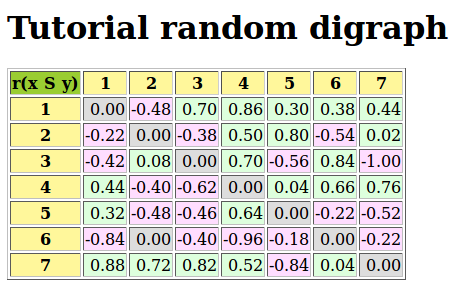
\includegraphics[width=7cm]{Figures/2-6-htmlTutorialDigraph.png}
\caption{The valued relation table shown in a browser window. Positive arcs are shown in green and negative arcs in red. Indeterminate --zero-valued-- links, like the reflexive diagonal ones or the link between node \texttt{'6'} and node \texttt{'2'}, are shown in gray}
\label{fig:2.6}       % Give a unique label
\end{figure}
 
\section{Complete, empty and indeterminate digraphs}
\label{sec:2.10}

Let us finally mention some special universal classes of digraphs that are readily available in the \texttt{digraphs} module\footnote{See \citealp{BIS-2021}}, like:
\begin{itemize}[nosep]
\item the \texttt{CompleteDigraph}\index{CompleteDigraph@\texttt{CompleteDigraph} class},
\item  the \texttt{EmptyDigraph}\index{EmptyDigraph@\texttt{EmptyDigraph} class} and
\item  the \texttt{IndeterminateDigraph}\index{IndeterminateDigraph@\texttt{IndeterminateDigraph} class} class,
\end{itemize}
who put all characteristic values respectively to the \emph{maximum}, the \emph{minimum} or the \emph{median} indeterminate characteristic value.
\begin{lstlisting}[caption={Complete, empty and indeterminate digraphs},label=list:2.11]
>>> from digraphs import CompleteDigraph,EmptyDigraph,\
...   			 IndeterminateDigraph
>>> # the empty digraph   
>>> e = EmptyDigraph(order=5)
>>> e.showRelationTable()
    * ---- Relation Table -----
      S   |    '1'    '2'    '3'    '4'	   '5'	  
    ---- -|-----------------------------------
    '1'   |  -1.00  -1.00  -1.00  -1.00	 -1.00	 
    '2'   |  -1.00  -1.00  -1.00  -1.00	 -1.00	 
    '3'   |  -1.00  -1.00  -1.00  -1.00	 -1.00	 
    '4'   |  -1.00  -1.00  -1.00  -1.00	 -1.00	 
    '5'   |  -1.00  -1.00  -1.00  -1.00	 -1.00
>>> e.showNeighborhoods() 
    Neighborhoods:
      Gamma     :
    '1': in => set(), out => set()
    '2': in => set(), out => set()
    '5': in => set(), out => set()
    '3': in => set(), out => set()
    '4': in => set(), out => set()
      Not Gamma :
    '1': in => {'2','4','5','3'}, out => {'2','4','5','3'}
    '2': in => {'1','4','5','3'}, out => {'1','4','5','3'}
    '5': in => {'1','2','4','3'}, out => {'1','2','4','3'}
    '3': in => {'1','2','4','5'}, out => {'1','2','4','5'}
    '4': in => {'1','2','5','3'}, out => {'1','2','5','3'}
>>> # the indeterminate digraph
>>> i = IndeterminateDigraph()
    * ---- Relation Table -----
      S   |   '1'   '2'	  '3'	'4'   '5'	  
    ------|------------------------------
    '1'   |  0.00  0.00	 0.00  0.00  0.00	 
    '2'   |  0.00  0.00	 0.00  0.00  0.00	 
    '3'   |  0.00  0.00	 0.00  0.00  0.00	 
    '4'   |  0.00  0.00	 0.00  0.00  0.00	 
    '5'   |  0.00  0.00	 0.00  0.00  0.00	 
>>> i.showNeighborhoods()
    Neighborhoods:
      Gamma     :
    '1': in => set(), out => set()
    '2': in => set(), out => set()
    '5': in => set(), out => set()
    '3': in => set(), out => set()
    '4': in => set(), out => set()
      Not Gamma :
    '1': in => set(), out => set()
    '2': in => set(), out => set()
    '5': in => set(), out => set()
    '3': in => set(), out => set()
    '4': in => set(), out => set()
\end{lstlisting}

Mind the subtle difference between the neighbourhoods of an \emph{empty} and the neighbourhoods of an \emph{indeterminate} digraph instance. In the first kind, the neighbourhoods are known to be completely \emph{empty}  (see List.~\vref{list:2.11} Lines 22-27) whereas, in the latter, \emph{nothing is known} about the actual neighbourhoods of the nodes  (see Lines 46-51). These two cases illustrate why in the case of \emph{bipolar-valued} digraphs, we may sometimes need both a \texttt{gamma} \textbf{and} a \texttt{notGamma} attribute.

\vspace{1cm}
In the following Chapter~\ref{sec:3}  we introduce the main formal object of this book, namely \emph{bipolar-valued outranking} digraphs.

%%%%%%%%%%%%%%%%%%%%%%%%%%%%%%%%%%%%
\phantomsection
\addcontentsline{toc}{section}{Notes}
\section*{Notes}

It is \emph{D. Bouyssou} \index{Bouyssou@\emph{D. Bouyssou}} who first suggested us end of the nineties, when we started to work in Prolog on the computation of digraph kernels with finite domain constraint solvers, that the $50\%$ criteria significance majority was a special value to be carefully taken into account. The converging solution vectors of the fixpoint kernel equations confirmed this special status of the $50\%$ majority (see Chap.~\ref{sec:17}). These early insights led to the seminal articles on bipolar-valued epistemic logic where we introduced split truth/falseness semantics for a multi-valued logical processing of fuzzy preference modelling \citep{BIS-2000,BIS-2002}. The characteristic valuation domain remained however the classical fuzzy $[0.0;1.0]$ valuation domain.

It is only in 2004, when we succeeded in assessing the stability of the outranking digraph when solely ordinal criteria significance weights are given, that it became clear and evident for us that the characteristic valuation domain had to be shifted to a bipolar $[-1.0;+1.0]$-valued domain \citep{BIS-2004a}. In this bipolar valuation domain, the $50\%$ majority thershold corresponds now to the median $0.0$ value, characterising with the correct zero value an epistemic indetermination --no knowledge-- situation. Furthermore, identifying truth and falseness by the sign of the characteristic values revealed itself to be very efficient not only from a computational point of view, but also from scientific and semiotical perspectives. A positive (resp. negative) characteristic value now attest a logically valid (resp. invalid) statement and a negative affirmation now corresponds to a positive refutation. Furthermore, the median zero value gives way to efficiently handling partial digraphs --like the border or the assymetric part of a digraph-- and, even more important from a practical decision making point of view, any missing data.

The bipolar $[-1.0;+1.0]$-valued characteritisc domain opened so the way to important new operations and concepts, like the disjunctive epistemic fusion operation seen in Section~\vref{sec:2.5} that confers the outranking digraph a logically and epistemically sound definition \citep{BIS-2013}. \Kendall 's ordinal correlation index could be extended to a bipolar-valued relational equivalence index between digraphs \citep{BIS-2012a}. Making usage of the bipolar-valued Gaussian error function naturally led to defining a bipolar-valued likelihood function, where a positive (resp. negative) value gives the likelihood of an affirmation (resp. a refutation) \citep{BIS-2014}.      

%%%%%%% The chapter bibliography
%\normallatexbib
%\clearpage
%\phantomsection
%\addcontentsline{toc}{section}{Chapter Bibliograhy}
\bibliographystyle{spbasic}
%\typeout{}
\bibliography{03-backMatters/reference}
%\input{02-mainMatters/02-chapterDigraphs.bbl}